%\input{|"curl -L 'https://virginia.box.com/shared/static/9120uqo655t0kwesti7t3exa7zsgbwdq.tex'"}
\include{article_header}
\title{Absence Makes the Ideal Points Sharper: Full-data IRT Models for Legislatures}
\usepackage{amsmath,amsthm, amssymb, latexsym}
\linespread{1.5}
\begin{document}
	
	\maketitle
	
	\begin{abstract}
		I put forward a Bayesian IRT model that can handle legislator absences and abstentions as additional data for determining legislator ideal points. The estimation uses the concept of a hurdle model to deflate the probabilities of legislator’s votes by the probability of absences. The model produces a single set of ideal points, but utilizes different parameters for bill absence midpoints. Compared to existing approaches, this model tends to produce more accurate estimates of ideal points for US Congresspeople who had higher rates of absence, such as senators on the campaign trail. For parliamentary data, the model provides much more precise estimates, especially in legislatures with very high rates of absence. Additionally, the model can incorporate absentions as a middle category between yes and no votes for legislatures with significant rates of abstentions.\footnote{I want thank Constanza Schibler,Jonathan Kropko and attendees at the 2017 Political Methodology Conference for helpful comments on this project. This paper is a working draft; please do not cite.}
	\end{abstract}
	
	Ideal point modeling of legislatures, and increasingly other kinds of social actors, has become a foundational element of empirical work in political science. However, most models of ideal points are based on binary outcomes that reflect yes and no votes (or positions) while all other actions are recorded as missing data. The argument for doing so is that the yes and no votes contain most of the information about legislator ideal points \parencite[4]{poole2008}, and that incorporating other categories such as abstentions or absences would greatly complicate the estimation without adding much benefit. In relation to the first point, I present a model that uses Bayesian Markov Chain Monte Carlo (MCMC) estimation to handle the contingency inherent in the data. In relation to the second, I show in this paper that absences and abstentions do contain important information about legislator ideal points, a contention that has become more prominent in recent research.
	
	However, I depart from the discussion of ideal point models in this recent literature by treating absences and abstentions as additional data rather than as missing yes/no votes. This distinction, while somewhat technical, has important ramifications for modeling choices. If absences and abstentions represent missing yes/no votes, then the solution is to impute how a legislator would have voted if they had not either been absent or voted to abstain. Accomplishing this result is no easy feat because multiple imputation methods require that at some level the unobserved outcomes be random, or ignorable, relative to the observed outcomes (i.e., yes/no votes). Given that legislator behavior is usually strategic and not random, I argue that the requirements of multiple imputation are unlikely to be met without relying on additional parametric assumptions. 
	
	This difficulty with multiple imputation, on the other hand, is in fact a feature rather than a bug because the observed outcomes--absence and abstention--offer potential insight into ideal points. To this end, I put forward a censoring approach to incorporate absences and abstentions by adding them as outcomes within a standard item-response theory (IRT) ideal point model. While the ensuing model is more complicated than a traditional ideal point model, the model estimates a single set of ideal points, which means that the ideal points will be more precisely estimated than with a model that uses only yes or no votes. By treating absences and absentions as additional observations of legislator behavior, rather than as a statistical problem to be overcome, ideal point models can produce new insights about legislators while utilizing existing rollcall data.
	
	In this paper I first describe the current state of ideal point modeling with an attention to the growing awareness of the problem of absences and abstentions. I then present the model formally and offer simulation results to verify the model's performance. Finally I examine two different empirical applications of the model, one drawn from data from the United States Congress and the second from the parliament in Tunisia's transitional democracy.
	
	\section*{Missing Data in Ideal Point Modeling}
	
	Following the pioneering work of \textcite{poole1997} and \textcite{jackman2004}, ideal point models have become a standard feature of the analysis of legislators and increasingly other political actors. The canonical ideal point model expresses legislator preferences as distances from a latent position in an $n$-dimensional policy space \parencite{enelow198} where the distances can be calculated either as Euclidean distances (IRT) or using the Normal distribution (i.e., the NOMINATE models), although both of these approaches tend to offer very similar estimates  \parencite{carroll2009}. A fully Bayesian analysis such as \textcite{jackman2004} is able to analyze virtually all bills, but whether done in a frequentist or Bayesian framework, the focus has remained on ideal points as representations of yes/no votes.
	
	Recently there has been criticism of these approaches because the ideal points that are estimated may not be an accurate measure of a legislator's ``true" ideological stance \parencite{krehbiel2014,Caughey2016,brauninger2016}. Statistically speaking, the ideal points are the dimension of variance that best explains the observed outcomes, so there is no easy way to know whether the ideal points refer to a legislator's ideological inclinations or more to her political strategies. For the model I present, however, this latter interpretation is more helpful because it makes it clear why data on absences and abstentions would be important to include.
	
	To the extent that voting can be represented in a unidimensional space, this space should be able to account for the full range of legislative behavior. The ideal point may properly refer to a legislator's firm political convictions or it may reflect his desire to appear more moderate/liberal/conservative for tactical reasons. Regardless, these ideal points are by definition the lowest-error explanation of observed behavior, and for that reason they are worth studying, even if as latent variables we cannot identify with complete certainty what social concepts they correspond to.
	
	Building on this work, political scientists have begun to look at alternative sources of data about ideal points beyond the collection of yes and no votes. A growing literature uses data generated outside of the legislature, whether via Twitter \parencite{barbera2015}, through political donations \parencite{bonica2014}, or through the legislator's prior history as a state representative \parencite{shor2011}. Most recently, \textcite{brauninger2016} and \textcite{rosas2015} have proposed methods for including abstentions and absences in parliamentary rollcall voting, while \textcite{powell2016} has presented new data on Congressional absences that shows how different types of absences may provide varying signals of legislator partisanship.
	
	What remains a lacuna, however, is how to incorporate absences and abstentions in the standard rollcall vote model that still serves as a benchmark for much of applied work in legislatures. The extant IRT models based on \textcite{jackman2004}, hereafter referred to as CJR, and the NOMINATE approaches \parencite{poole2008} drop absences and absentions from their data, which means that the ideal points ignore any information contained in this part of the dataset. Properly speaking, the standard models are only defined over the subset of rollcall voting that comprises yes and no votes. It is not that these models are in any sense incorrect, but rather that their domain is limited to the binary relationship of opposing votes on bills. However, it would seem that given the interest in obtaining new methods of ascertaining ideal points, we should look at the full range of vote records available in roll-call datasets.
	
	
The methodology that has been used so far to address this problem is multiple imputation because absences and abstentions are coded as missing values. Multiple imputation involves estimating the distribution of possible yes or no votes to replace all of the absences and abstentions in the data. Crucially, for this method to work, the probability of an unobserved response must not depend on the value of that unobserved response \parencite{rubin2002}. 	In the broader IRT field there are extant approaches to handling missing data that follow from \textcite{rubin2002}'s framework. \textcite{mislevy2016} provides a helpful summary of these approaches by showing how ignorability of missing data, and the crucial missing-at-random (MAR) assumption, depends on the relationship between the person ``ability" parameters (i.e., legislative ideology) and the item parameters (i.e., bill yes/no points). However, he concludes that if the missing data is due to ``intentional ommission" or to ``examinee choice", then no extant IRT missing-data model is able to meet the MAR assumption (p. 192). However, virtually all recorded legislative actions are intentional at some level. To correctly impute votes, we would need to imagine a counter-factual world in which some divine force forced a legislator to show up and then to vote either yes or no. While this counterfactual is plausible in some situations, such as if a legislator suffered some kind of accident preventing her from showing up, in general it is not plausible to impute this counterfactual.
	
	However, this approach can be used within the context of a specific model specifying how the counterfactual could occur. \textcite{rosas2015} is the first to apply this theoretical approach to rollcall voting data via an imputation model of legislative behavior framed in terms of disagreement between a party member and the party's official position.  As \textcite{rosas2015} point out, in the case of rollcall vote data, the assumption that absences and abstentions can be thought of as a plausibly random distribution yes/no votes is unlikely to be true. In \citeauthor{rosas2015}'s model, yes and no votes are imputed based on whether a party member is in agreement with his or her party given the assumption that, conditional on knowing whether a party member is in disagreement, the ensuing decision to vote yes or no only depends on observed ideal points \parencite{rubin2002}, and hence is imputable. This model provides a compelling account of how a legislator may decide to abstain in a vote; however, the model's applicability is also limited to this specific counterfactual. For example, \citeauthor{rosas2015} collapse both absences and abstentions into a single category because in their framework these actions are equal signals of party disagreement, but this may not be applicable to other situations of legislative behavior.
	
	By comparison, the model that I propose should apply to abstention and absence data more broadly, although it does not provide special insight into intra-party dynamics as \textcite{rosas2015} do. The main difference is that I do not attempt to impute observations. Rather, the model I present in this paper treats absences and abstentions as additional data that can estimated jointly with the standard models to improve the accuracy of ideal points. By treating absences and abstentions as strategic actions, I can directly incorporate them into the model as additional evidence of legislators' ideal points. This change in focus allows for a complete-data IRT model that uses every possible category of votes (absent, abstain, yes, no) in legislative roll-call datasets.
	
	
	
	\section*{Absence-Inflated Hurdle Model}
	
 	To construct this model, I first return to the canonical treatment of ideal point models in \textcite{enelow198}. In the elementary spatial model that is the foundation of the statistical ideal point literature, a legislator $x_i$ votes for a bill if the yes position $y$ on the bill is closer to $i$ than the no position $n$ on the bill: $\mid x_i-y \mid > \mid x_i - n \mid$, and the legislator is indifferent if the difference in utilities is exactly equal: $\mid x_i-y \mid = \mid x_i - n \mid$. In statistical terms we can imagine legislators having a stochastic ideal point function that can be represented as a normal curve or as a quadratic function \parencite{carroll2009}. This standard form of the model is represented by Figure \ref{ehinich} in which the ideal point $x_i$ is represented by a normal distribution over the possible utilities and the bill positions by vertical lines.
 	\begin{figure}[h!]
 		\caption{Standard Ideal Point Model of \textcite{enelow198}}\label{ehinich}
 		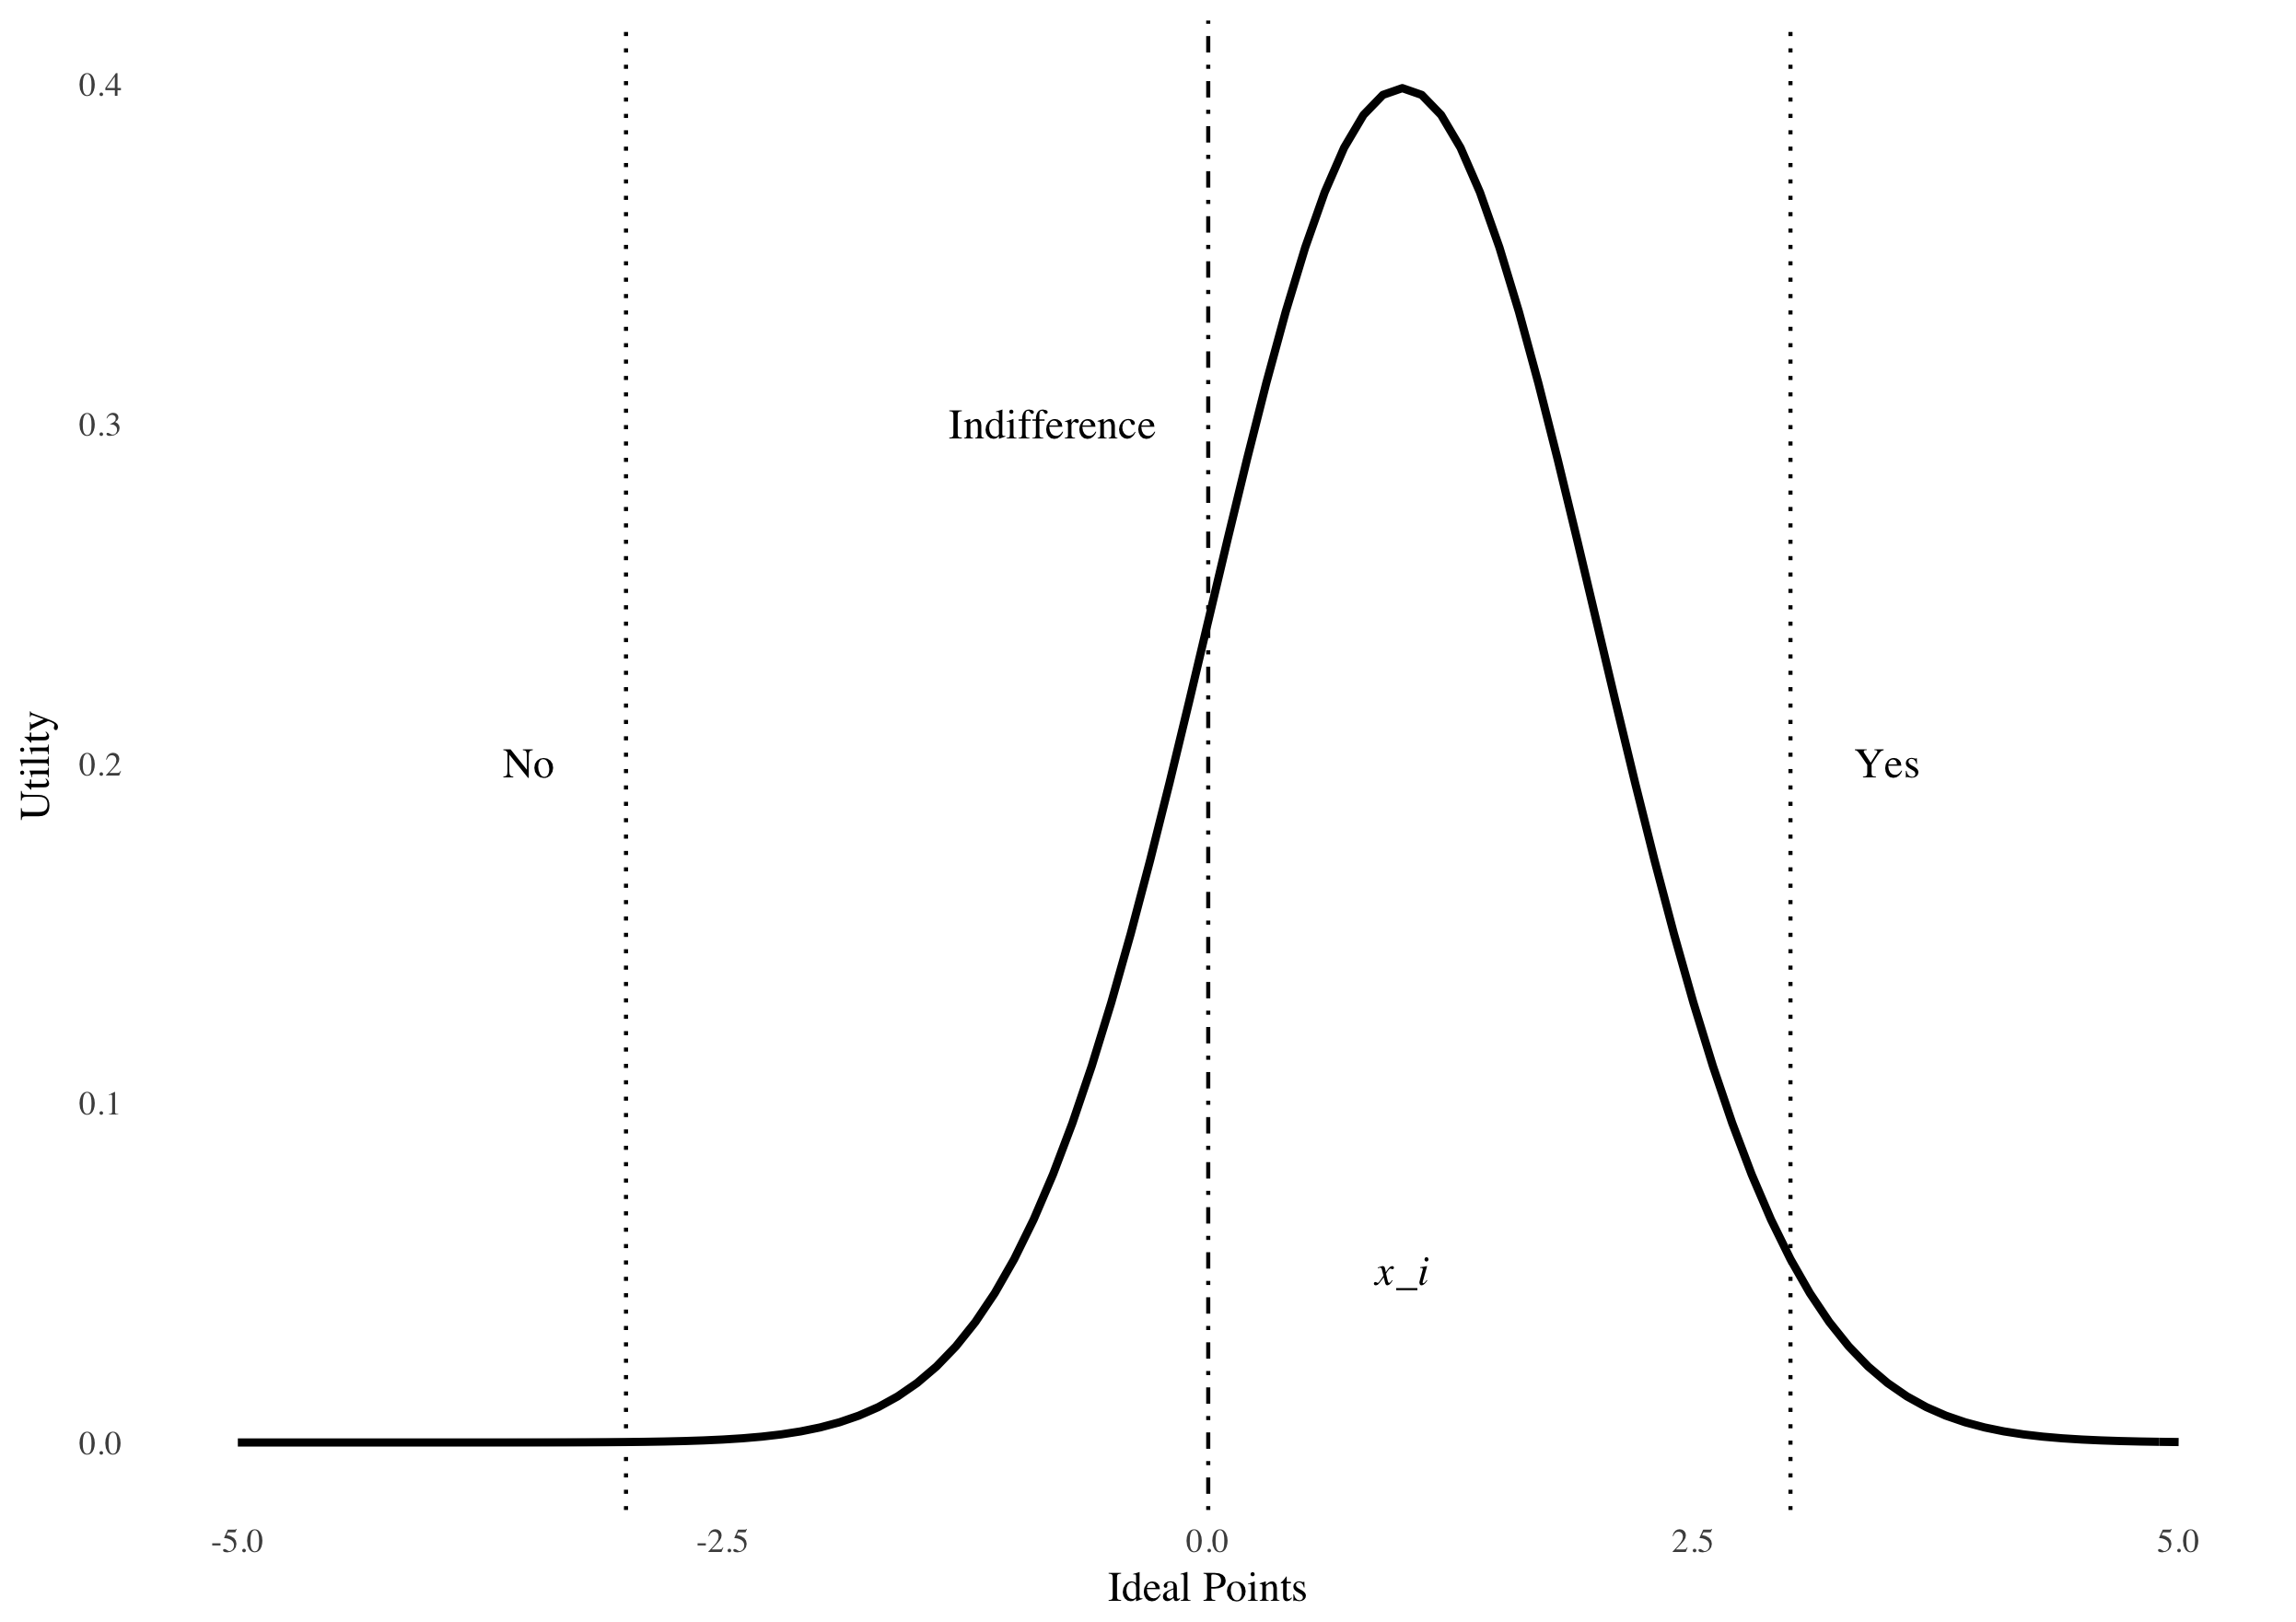
\includegraphics[width=0.9\linewidth]{standard_ideal_pt}
 	\end{figure}
 
 	The first step in building a model that can handle both absences and abstentions is to modify how the legislator responds to an additional vote choice: abstention. Two approaches exist: 1) abstain, yes and no could be unordered positions for each bill such that each vote position could take any position along the ideal point scale, or 2) an ordinal function in which the abstain point must be between yes and no positions. I argue that the latter is the correct approach for ideal point models because of the original intention behind the model's design. In order for the positions of the bills to represents preferences over policy outcomes, a vote of yes or no must become increasingly likely as the ideal point scale moves toward positive or negative infinity. Otherwise the model will start to address non-policy concerns such as vote trading and other forms of legislative strategy if either end of the ideal point spectrum is associated with abstention instead of a distinct yes or no vote. 
 	
 	Suppose, for example, that a legislators were deciding a military funding bill. If the abstention point was further to the right or left than either the yes or no points, it would be plausible for hawks or doves to become less likely to vote for the bill as military spending increased or decreased. While such outcomes certainly do occur in legislators due to legislative strategy taking predominance over specific policy goals, such a model would depart significantly from a clear and useful interpretation of ideal points as a reflection of the policy space.
 	
 	With an ordering of votes, however, the original meaning of the ideal point remains intact, albeit with additional complexity. A revised version of the model can be seen in Figure \ref{abs_pts}. The addition of an absention point for the bill in between the yes and no votes produces a zone in which a legislator with an ideal point within that zone is more likely to abstain than to vote yes or no. Instead of one indifference point, there are now two indifference points where a legislator $x_i$ could be indifferent between abstaining and voting no and abstaining and voting yes. In this figure, the legislator has a higher probability of voting abstain followed by a yes vote and then a no vote.
 	 	\begin{figure}[h!]
 		\caption{Revised Ideal Point Model with Abstention}\label{abs_pts}
 		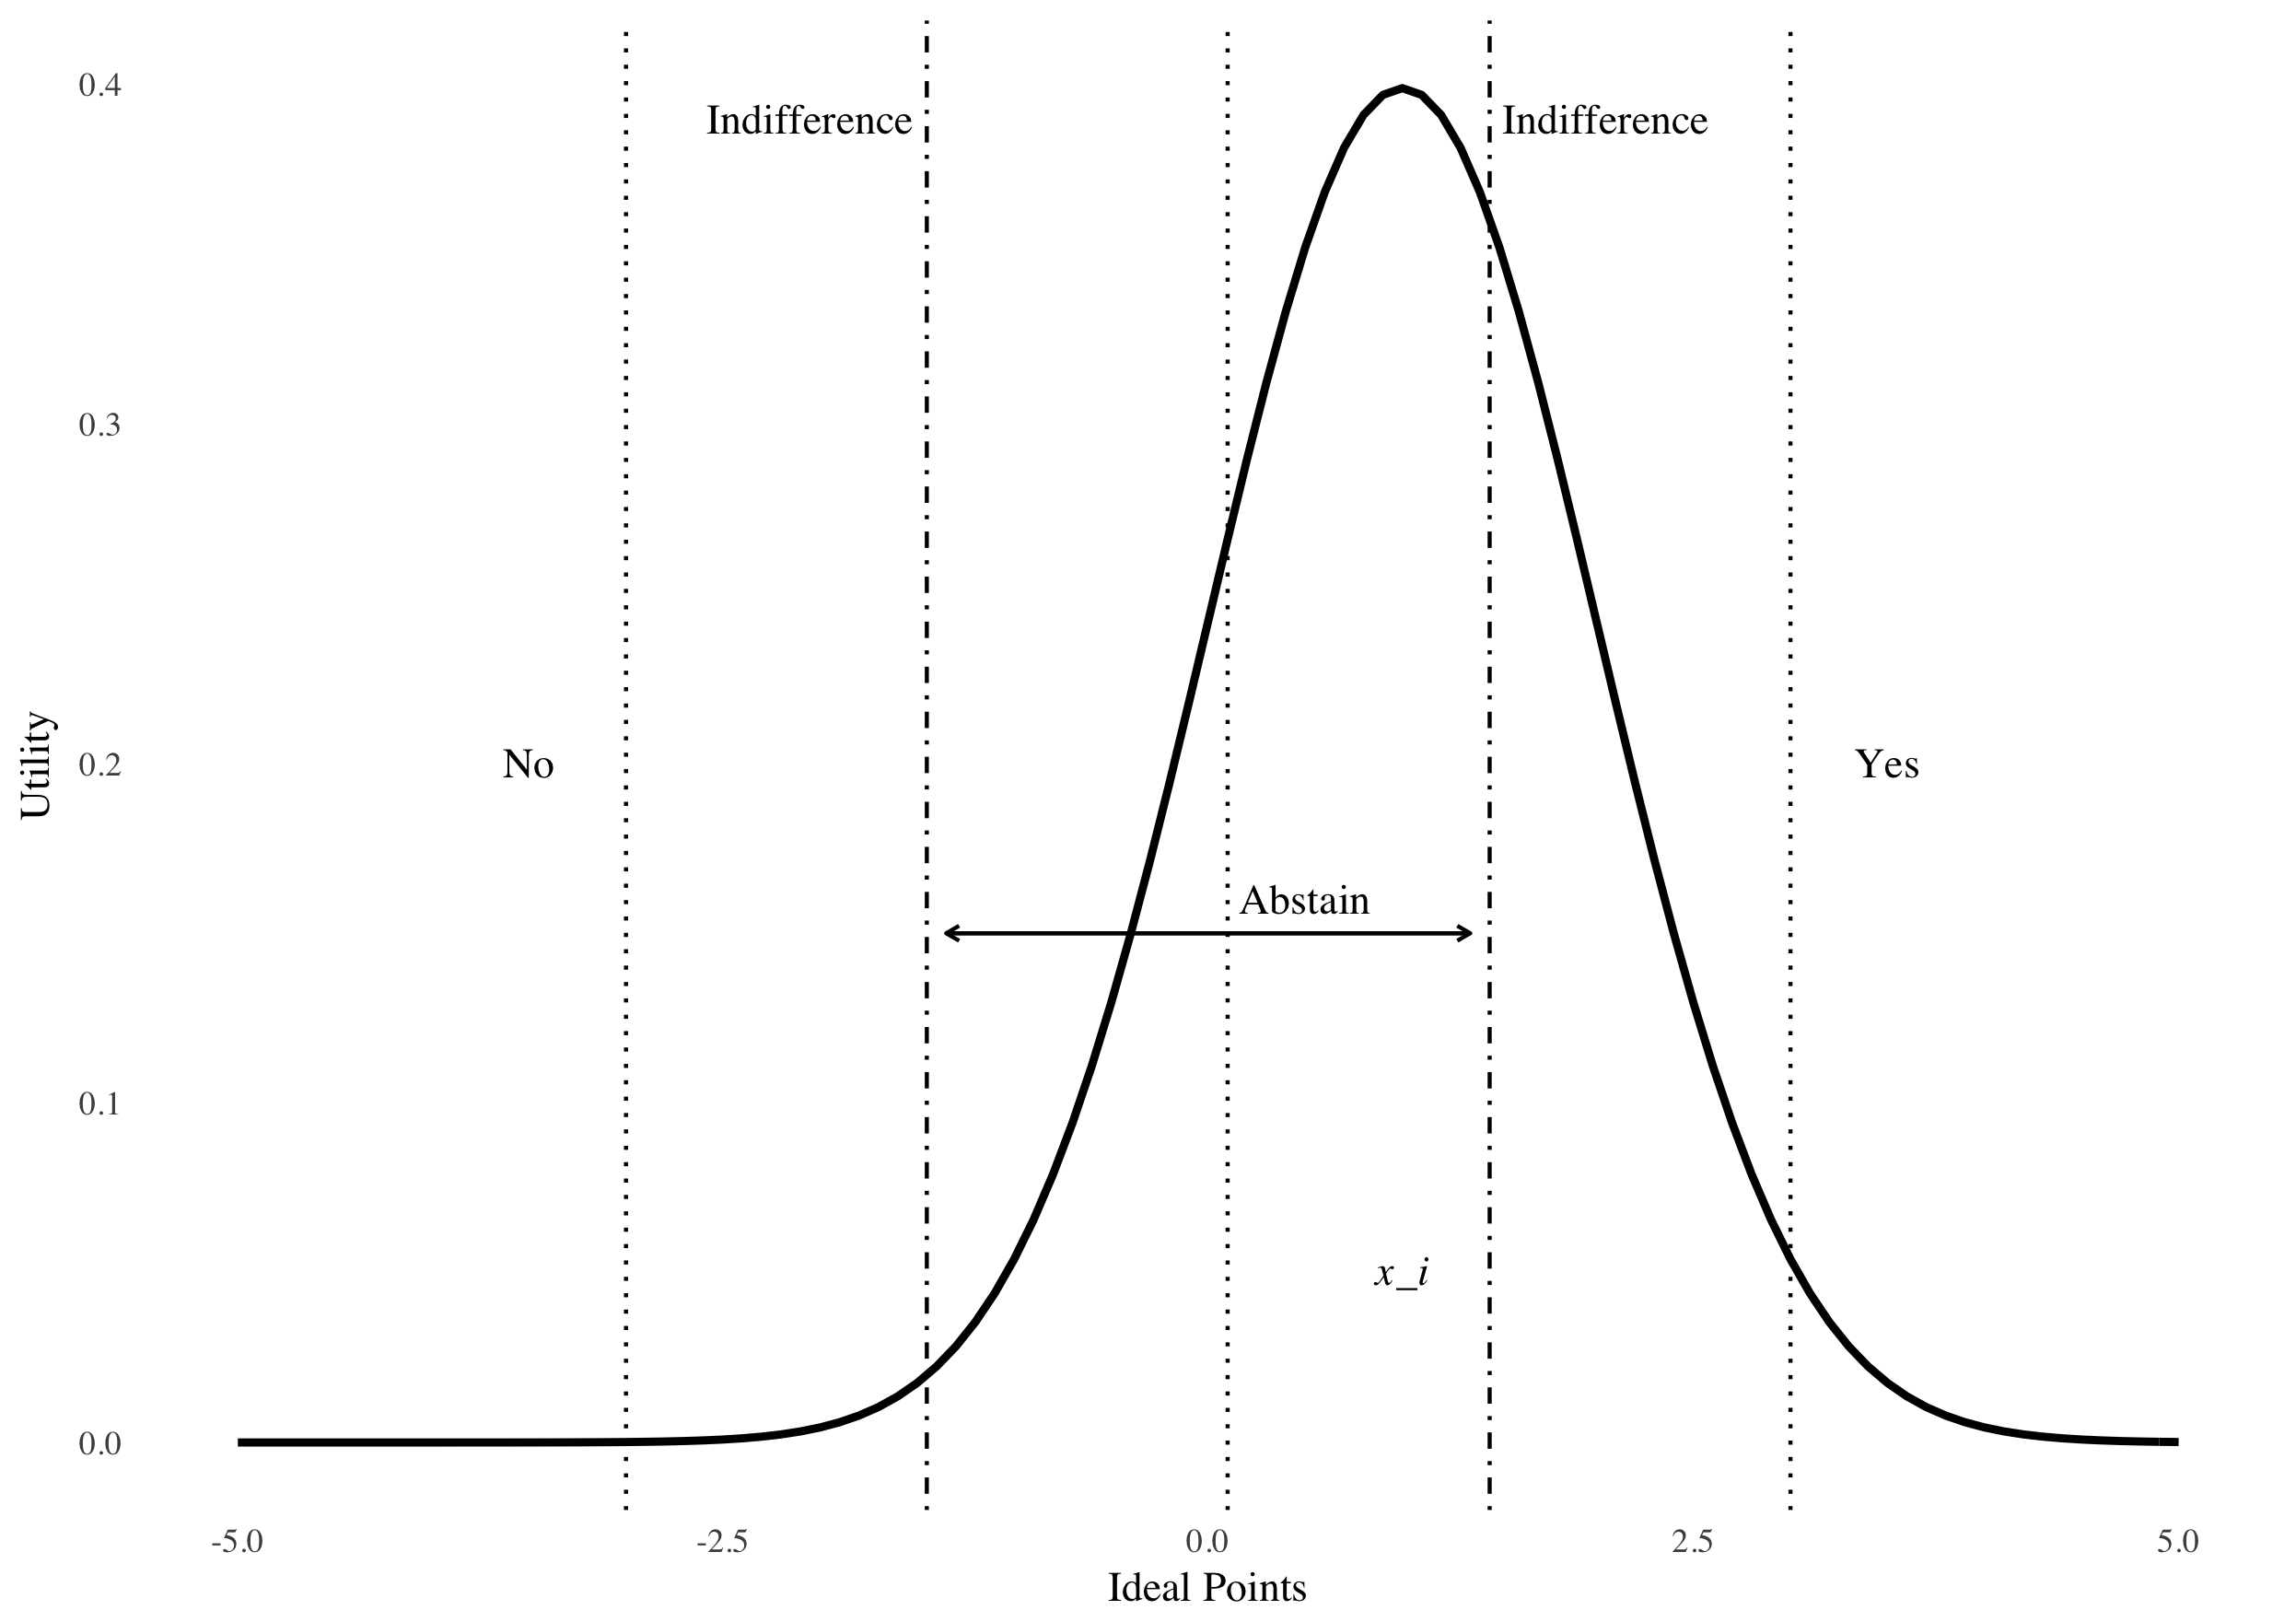
\includegraphics[width=0.9\linewidth]{ideal_pt_with_abstain}
 	\end{figure}
	
This formal model can be directly translated into an ordinal IRT model, which is known as a rating-scale model in the IRT literature.\footnote{A rating-scale model has fixed cutpoints for the entire data and matches the parameterization of the commonly-used ordered logit model. The graded-response model, on the other hand, estimates separate cutpoints for each bill. While it is an interesting extension of the basic model, it is not considered in this paper, although it can be estimated in the \texttt{idealstan} R package.} The $K$ category vote outcome $k$ can be modeled as a likelihood function $L(\cdot)$ of $I$ legislator ideal points $x_i$, $J$ bill discrimination parameters $\beta_j$ and $J$ bill intercepts $\alpha_j$. Each equation is put inside $\zeta(\cdot)$, which represents the logit function. Formally, the full likelihood is:
	
					\[
	L(\beta,\alpha,x|Y_{k}) = \prod_{n}^{i=1} \prod_{m}^{j=1}
	\begin{cases} 
	1 -  \zeta(x_{i}'\beta_j - \alpha_j - c_1) & \text{if } K = 0 \\
	\zeta(x_{i}'\beta_j - \alpha_j - c_{k-1}) - \zeta(x_{i}'\beta_j - \alpha_j - c_{k})       & \text{if } 0 < k < K, \text{ and} \\
	\zeta(x_{i}'\beta_j - \alpha_j - c_{k-1}) - 0 & \text{if } k=K
	\end{cases}
	\]
	
	The use of $K$ ordered outcomes allows the model to incorporate abstentions as a third category between yes and no votes. Because the cutpoints are estimated from the data, the actual width of the utility apportioned to voting in each category will vary from dataset to dataset. In the Bayesian framework with priors on variables described later, there is no risk of cutpoint collapse because any bills with zero abstentions will simply default to the prior.
	
	The bill intercepts also have a slightly different interpretation in this model. The intercept for each bill is actually $\alpha_j + c_k$ for all $K$ so that in effect the bill has an intercept for each category of vote outcome. Otherwise, however, the estimated parameters are interpreted identically to the standard IRT model \parencite{jackman2004}. The $x_i$ represent legislator ideal points, and the bill midpoints (i.e., the line of indifference for each vote outcome) are equal to $\frac{\alpha_j + c_{k-1}}{\beta_j}$. Thus for a rollcall voting model with three distinct outcomes, yes, no and abstain, there will be two lines of indifference (or equiprobability contours) for each bill that separate legislators into groups that are more or less likely to vote in each vote category. For the binary case in which $K=2$, the cutpoints collapse into the bill intercepts and a standard binary logit model is estimated.
	
	In order to model absences, this standard IRT model is embedded within a hurdle framework, which is similar to the zero-inflated models popular with handling over-dispersion in count data \parencite{zorn1998}. We assume that the probability that a legislator is absent is equal to $r$ and the probability that the legislator shows up to vote is equal to $1-r$. The probability $r$ is itself modeled as a binary IRT model in which the ideal points $x_i$ are shared with the vote equation while the bills receive separate parameters $\gamma_j$ for discrimination and $\omega_j$ as intercepts. Functionally, this means that the probability of any vote $k$ is decreased proportionally as the probability of absence $r$ increases. A legislator will only vote if the hurdle of strategic absence is overcome. That is to say, not only does each bill have a point in a voting ideal space, it also has a point in an absence ideal space that is also relative to the legislators' own ideal points.
	
	The combined model is as follows:
	
		 \[
	L(\beta,\alpha,X,Q,\gamma,\omega|Y_{k},Y_{r}) = 
	\prod_{n}^{i=1} \prod_{m}^{j=1}
	\begin{cases}
	\zeta(x_{i}'\gamma_j - \omega_j ) & \text{if } r=0, \text{ and} \\
	(1-\zeta({x_{i}'\gamma_j - \omega_j}))L(\beta,\alpha,X|Y_{k1}) & \text{if } r=1
	\end{cases}
	\]
	
	Substantively, the additional bill parameters $\gamma_j$ and $\omega_j$ represent the position in the ideal point space of the salience of a particular bill. $\omega_j$ refers to the average probability that legislators will be absent on a given bill, while $\gamma_j$ reflects the position in which the bill is pointing in the ideal space, i.e., whether a bill is liberal or conservative. Unlike in standard IRT models,the $\gamma_j$ and $\beta_j$ discrimination parameters are unconstrained to allow a bill to have either a conservative or liberal polarity in the ideal point space. 
	
	The addition of parameters, and the dependent relationship between the hurdle model and the vote model, makes estimation more challenging. Estimating the parameters with Bayesian MCMC requires the usual identification restrictions on parameters \parencite{jackman2004,gelman2005}, but the additional parameters may require further constraints in order to identify the model. There is no easy or straightforward method to identify this model as it depends in part on the presence of information in the model about both bills and legislators. However, the usage of usual identification methods, such as constraining polarity and fixing parameters is able to identify most models.\footnote{In the R package \texttt{idealstan} I provide methods for automatically identifying models through the use of variational Bayesian inference} For the purposes of this paper, I identify models by constraining the polarity of legislators, using informative priors and also fixing one bill intercept to zero.
	
	The following priors are put on all of the parameters:
	
	\begin{align*}
		c_k - c_{k-1} &\sim N(0,5)\\
		\gamma_j &\sim N(0,2)\\
		\omega_j &\sim N(0,5)\\
		\beta_j &\sim N(0,2)\\
		\alpha_j &\sim N(0,5)\\
		x_i &\sim N(0,1)
	\end{align*}

	
	Essentially, the intercepts and discrimination parameters are given a weakly informative priors ($N(0,5)$ and $N(0,2)$ represent the full range of probabilities on the logit scale). For scale identification purposes, the $x_i$ ideal points are given a $N(0,1)$ prior. In addition, one each of the $\alpha_j$ and $\omega_j$ intercepts are fixed at zero in order to prevent scale shifts in the parameters. A prior is put on the difference between the cutpoints $c_k$ rather than on the cutpoints themselves because it is difficult to affix concrete values to cutpoints a-priori, although the differences between cutpoints can be weakly identified. The prior on the cutpoints prevents cutpoint collapse so that it is not necessary to have a certain number of abstentions for each bill, while the bias of using a weakly informative prior is minimal.
	
	To show how the model performs, I simulated data of 50 legislators and 50 bills. For the purposes of identification, I constrained the signs of ten legislators to identify the scale, and used vague priors on the other parameters as mentioned above. In addition, one of the bill intercepts is set at zero to prevent scale shifts. Estimation of the model was through an R package \texttt{idealstan} that provides this model along with other absence-inflated IRT ideal point models for both ordinal and binary data with the underlying MCMC done via the Stan engine \parencite{carpenter2017}. The results of the simulation are shown in Figure \ref{sim_results}. As can be seen, the model is able to recover the true parameters on average, and the 5\%-95\% high posterior density intervals (HPD) also cover the true values. Generally speaking, the model is better able at recovering the relative positions of the parameters rather than their true values, as ideal point models are only identified up to a rotation or scaling of the associated ideal points \parencite{gelman2005}. However, the use of the tight priors on the ideal points, combined with zeroing a bill intercept, is generally able to return the ``true" values of the parameters. In the more likely situation in which the choice of scale is arbitrary, the priors can be adjusted without changing the interpretation of the model's results. 
	
	\begin{figure}
		\caption{True and Estimated Values}\label{sim_results}
		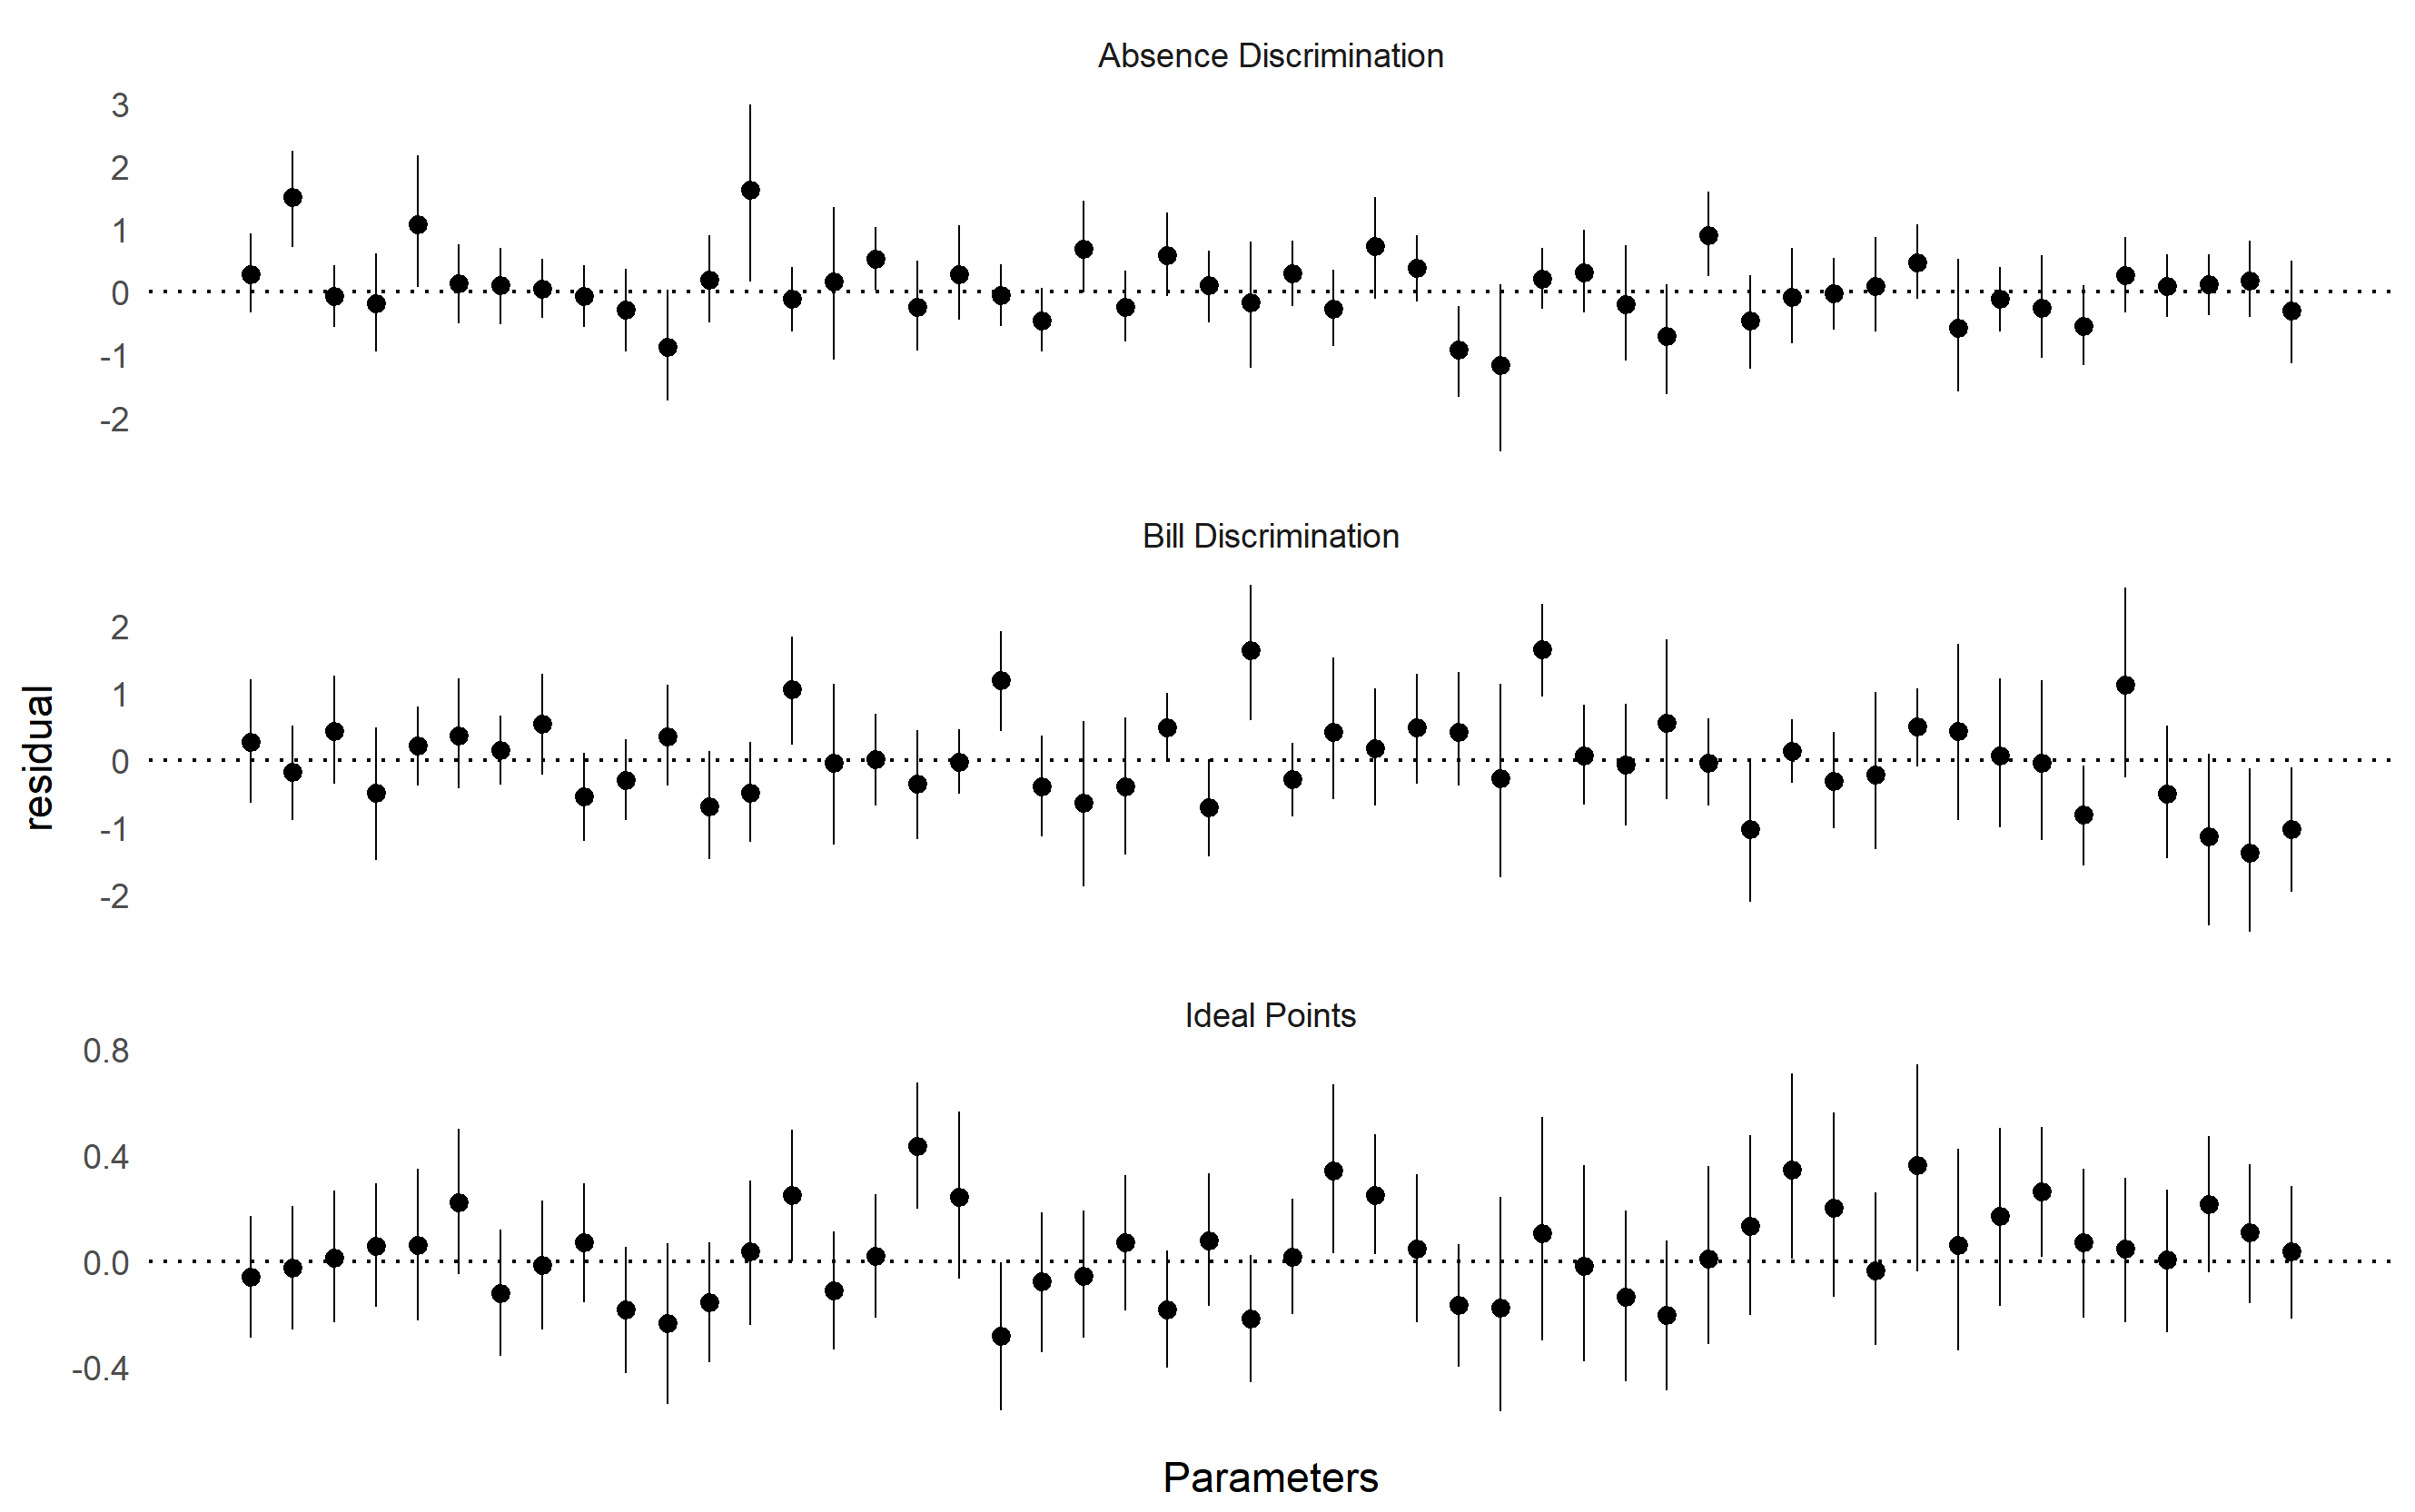
\includegraphics[width=\linewidth]{param_resid}
	\end{figure} 
	
	The use of simulated data is also helpful for evaluating the difference between the standard ideal point models and the ``true" absence-inflated model. This test is of course arbitrary as the data were generated to conform to absence-inflation, but it still a helpful way to diagnose potential model misfit. After estimating separate models for CJR and W-NOMINATE, I standardized all the values to remove any scale differences and then calculated RMSE for all the legislator ideal points relative to the true values. These results are shown in Figure \ref{sim_rmse}. While it is unsurprising that the RMSE for the absence-inflated model is quite low, it is interesting to note that W-NOMINATE shows slightly less bias than CJR, which is odd considering that the CJR model is substantively more similar to the absence-inflated IRT model than is W-NOMINATE. However, this could simply be an artifact of the W-NOMINATE estimation dropping three legislators because they did not have enough yes or no votes. In any case, for this simulation, at least, the level of bias appears to be approximately 40 percent greater than the correct estimator, which is also close to the proportion of absences and abstentions in the simulated dataset (52.4\%). In general, in line with \textcite{rosas2015}, we would expect this kind of bias to increase in proportion to the number of votes dropped from the ideal point estimation so long as the choice to show up to vote is strategic and not based on exogenous factors.
	
	\begin{figure}
		\caption{RMSE for All Models}\label{sim_rmse}
		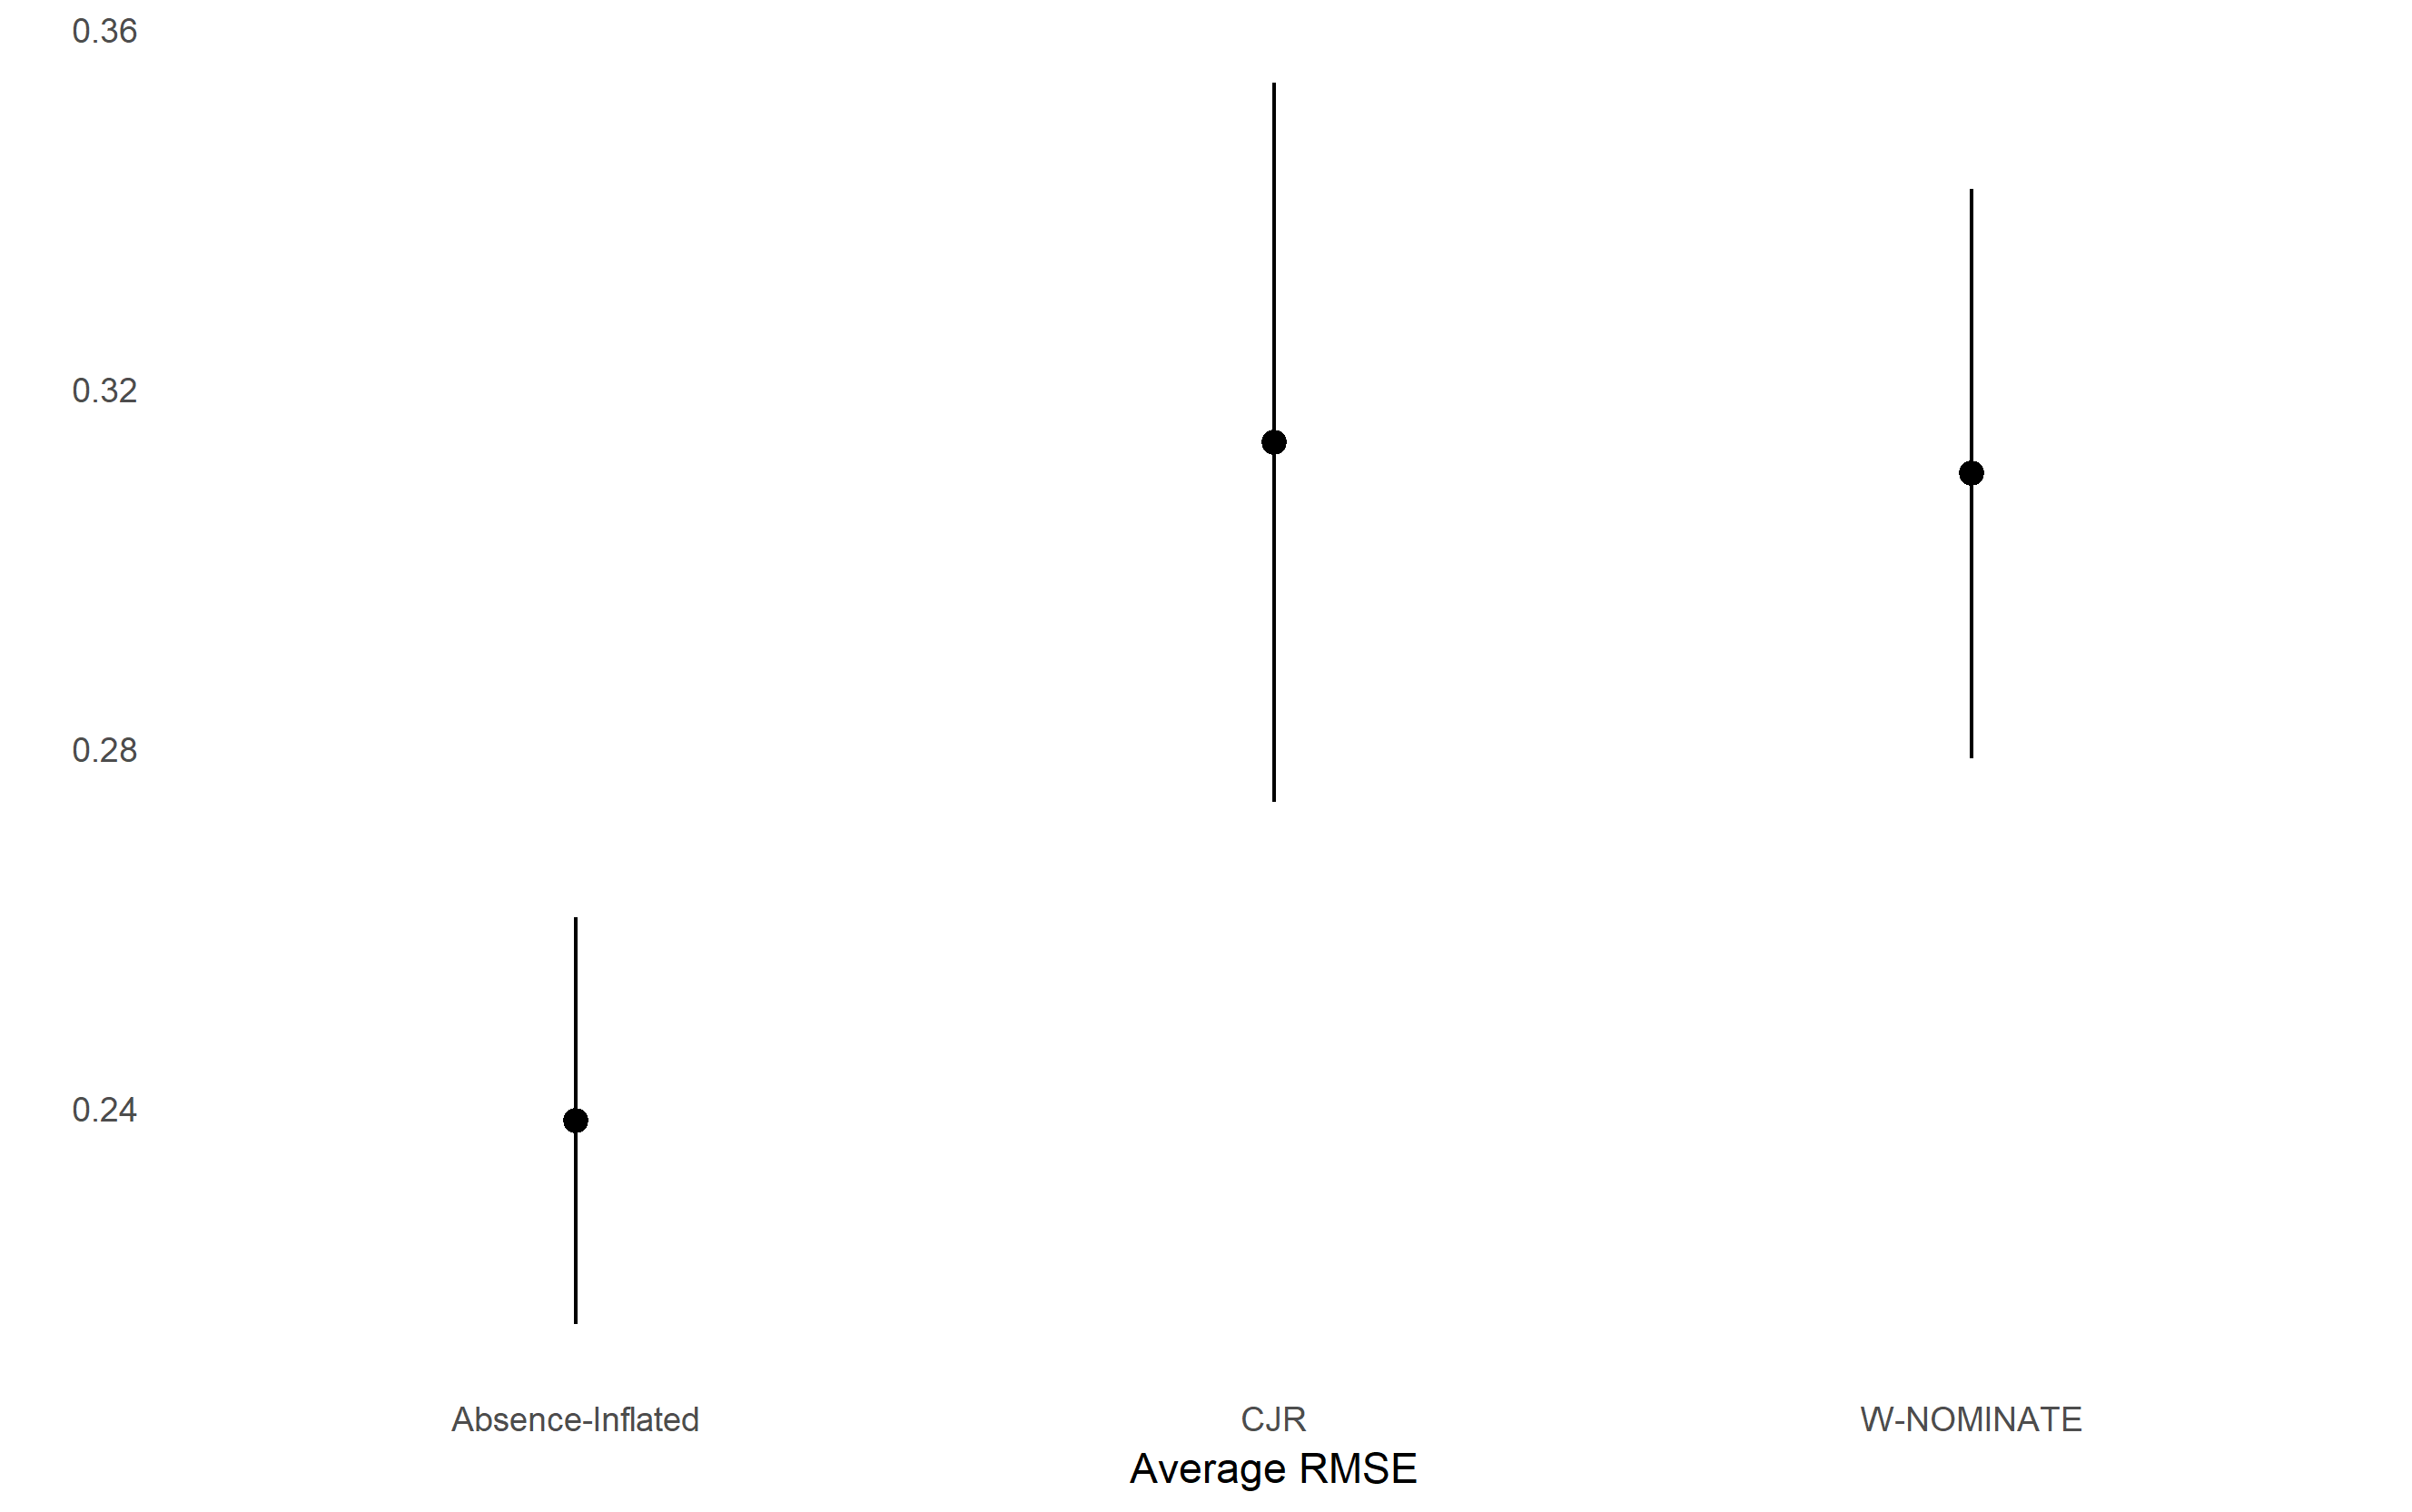
\includegraphics[width=\linewidth]{sim_rmse_allmods}
	\end{figure} 
	
	
	\section*{Empirical Applications}
	
	As an empirical application of the model, I look at two rollcall datasets, one from the 114th Senate and the second from a transitional democracy, Tunisia. For both datasets I use existing R packages, \texttt{wnominate} and \texttt{pscl}, to obtain ideal scores using the W-NOMINATE and CJR methods respectively. I then estimated absence-inflated models for both datasets, a binary IRT for the Senate data and an ordinal IRT for the Tunisian data. I did not use an ordinal model for the Senate data because there were only a handful of abstentions in the 114th Senate, and estimating cutpoints for abstention would make little difference to the model. All of the results were standardized to ensure that arbitrary scale shifts did not affect comparisons.
	
	\subsection*{US Congress}
	
	The estimation results for the 114th Senate show that overall the absence-inflated model and both CJR and W-NOMINATE correlate very highly, as might be expected given the relatively low rates of absence. Figure \ref{compare_con} reveals that the models tend to diverge only in the tails of the Republican and Democrat parties. Furthermore, although the absence-inflated model is structurally more similar to CJR in that it is based on an IRT framework, for some legislators the absence-inflation model is closer to W-NOMINATE's estimate. 
	
	\begin{figure}
		\centering
		\caption{Comparison of Ideal, W-NOMINATE and Absence-Inflation Models for 114th Senate}\label{compare_con}
			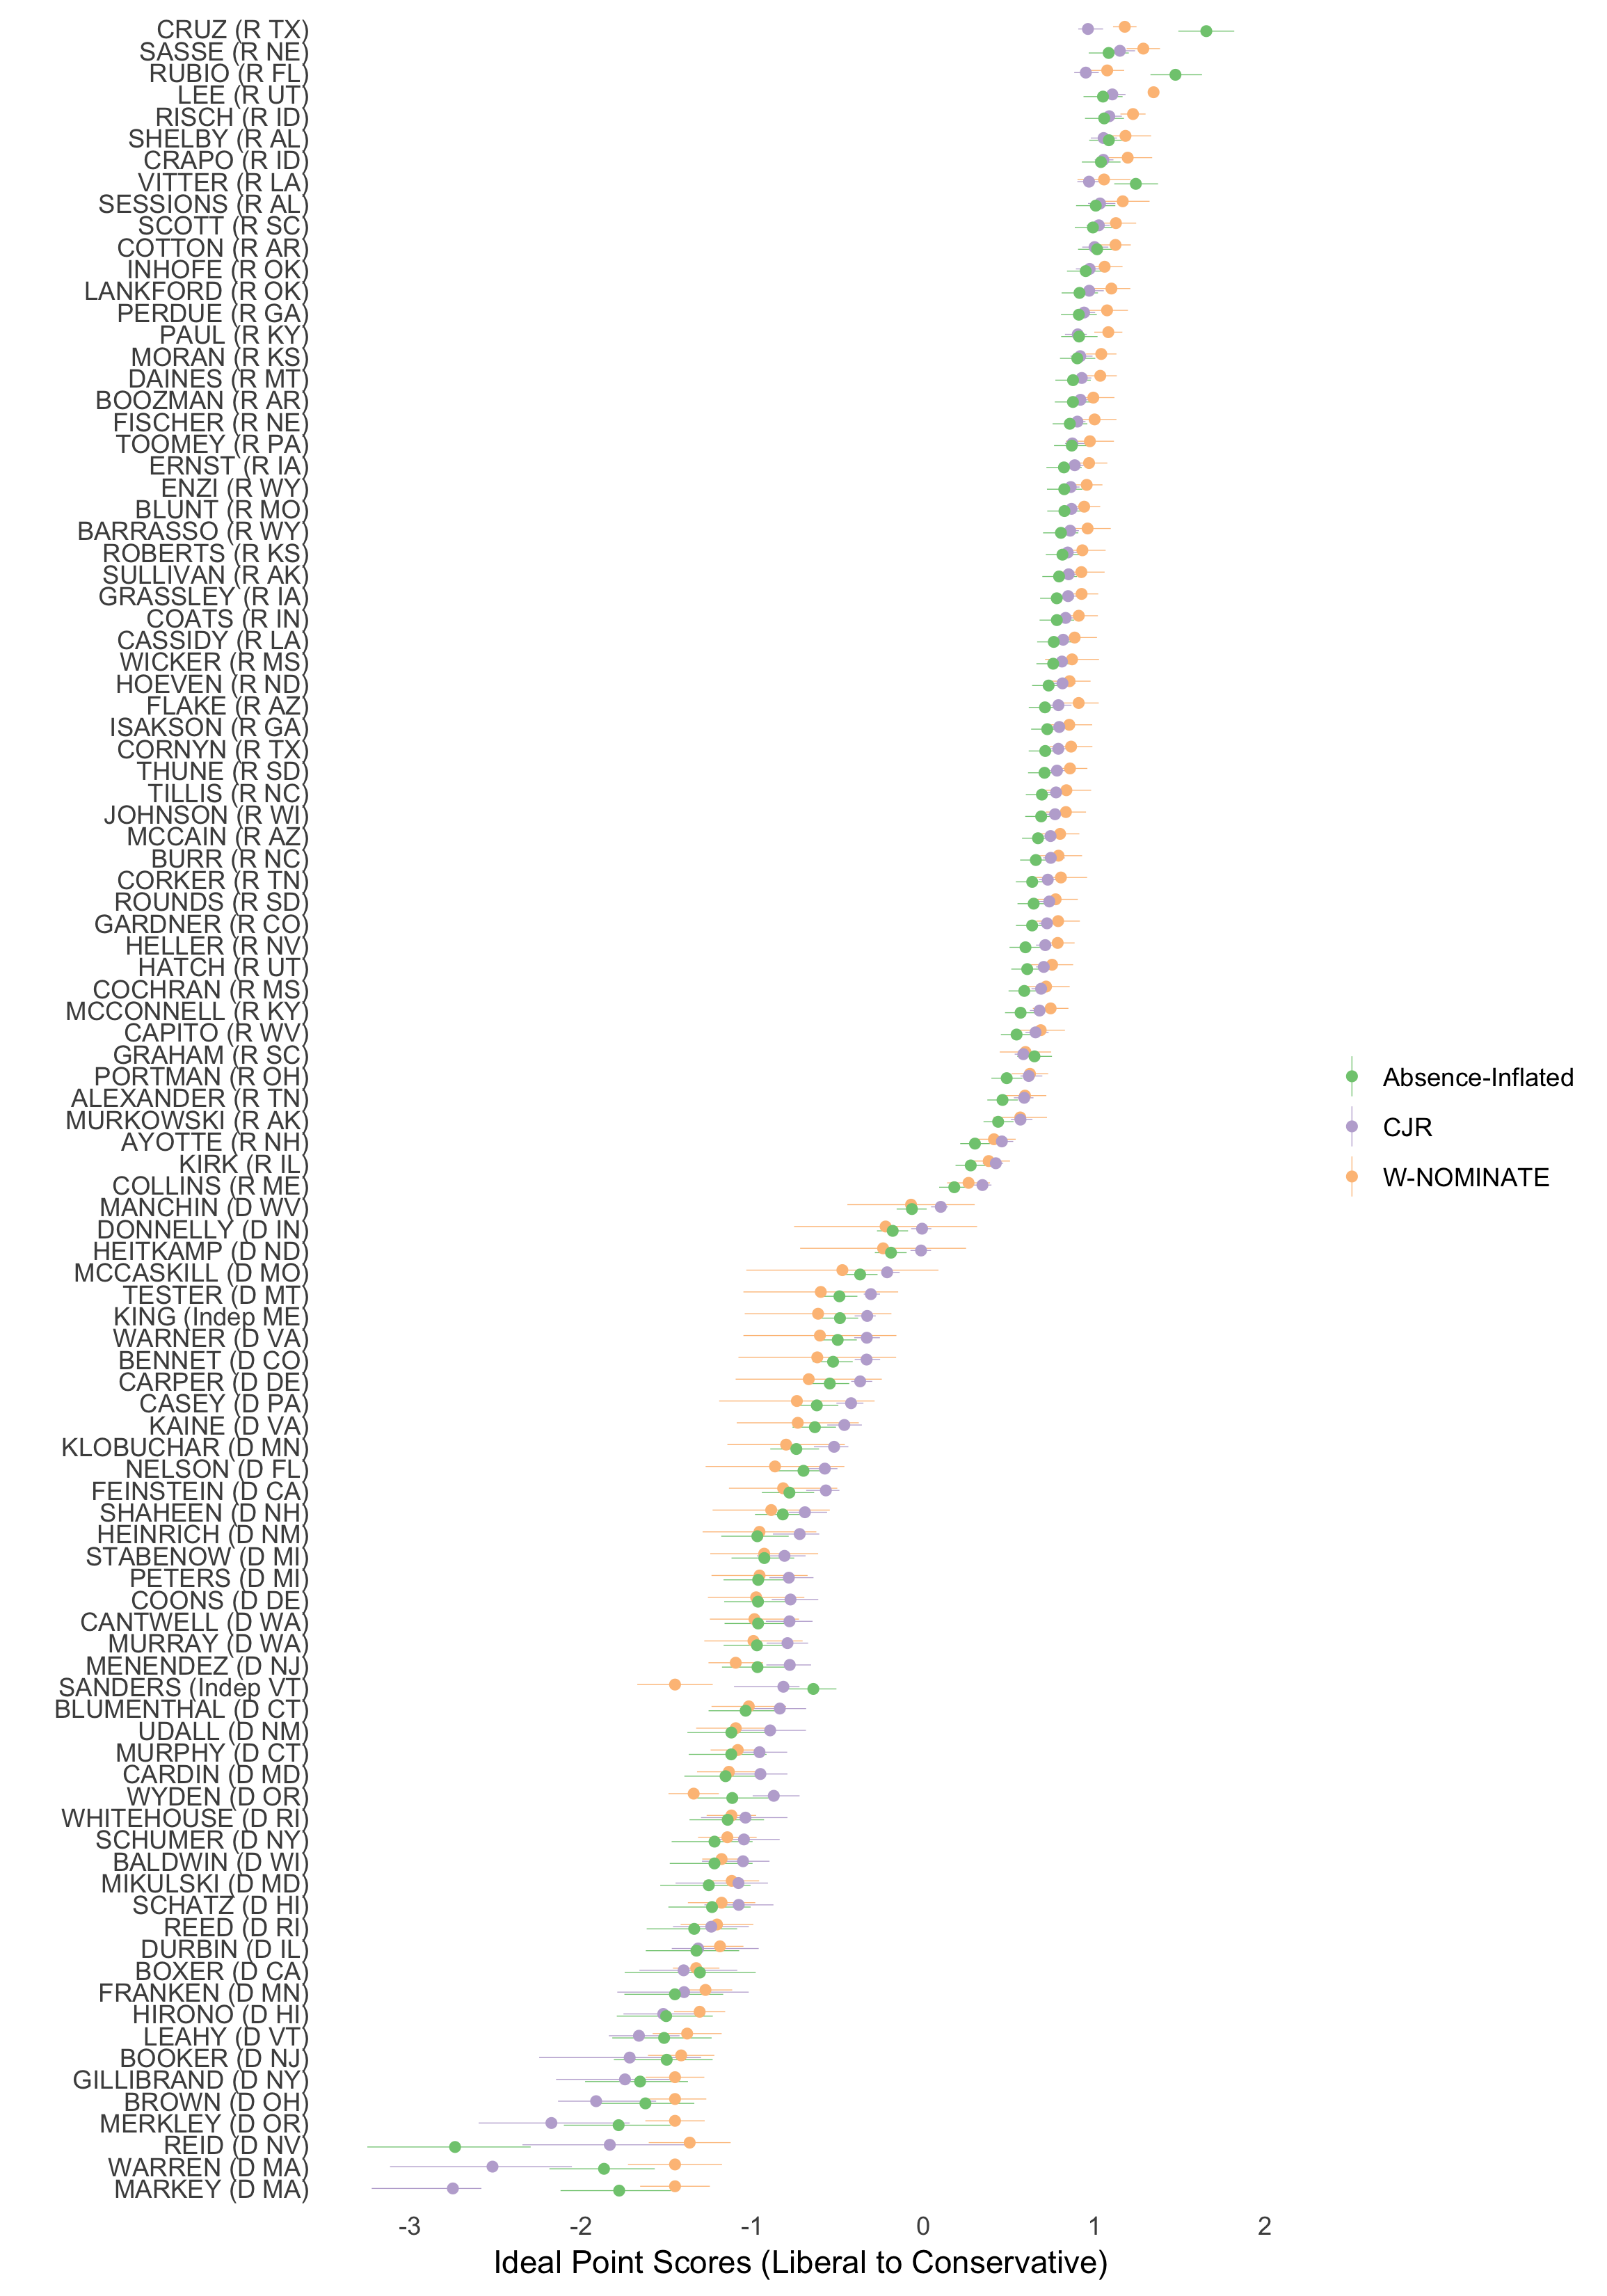
\includegraphics[width=\linewidth]{all_perf}
	\end{figure}
	
	Figure \ref{compare_con} shows that the standard models of CJR and W-NOMINATE are quite accurate at capturing ideal points despite the fact that these models drop absences. The close correlation between the scores shows that even if the assumptions of these models are not met, the resulting estimates are still very usable because the low number of absences ensures the model is still a close approximation of reality. However, as may be expected, the estimates diverge for those legislators who have higher rates of absence. For the 114th Senate, these are primarily Senators who were competing in the presidential primaries: Bernie Sanders, Ted Cruz and Marco Rubio. In fact, the absence-inflation model shows Ted Cruz and Marco Rubio as the most conservative senators in the data set, which is likely because Cruz and Rubio made sure they showed up for votes that mattered to the conservative Republican base during the primary season.
	
	\begin{figure}
		\centering
		\caption{Rank Changes for 114th Senate}\label{rank_sen}
		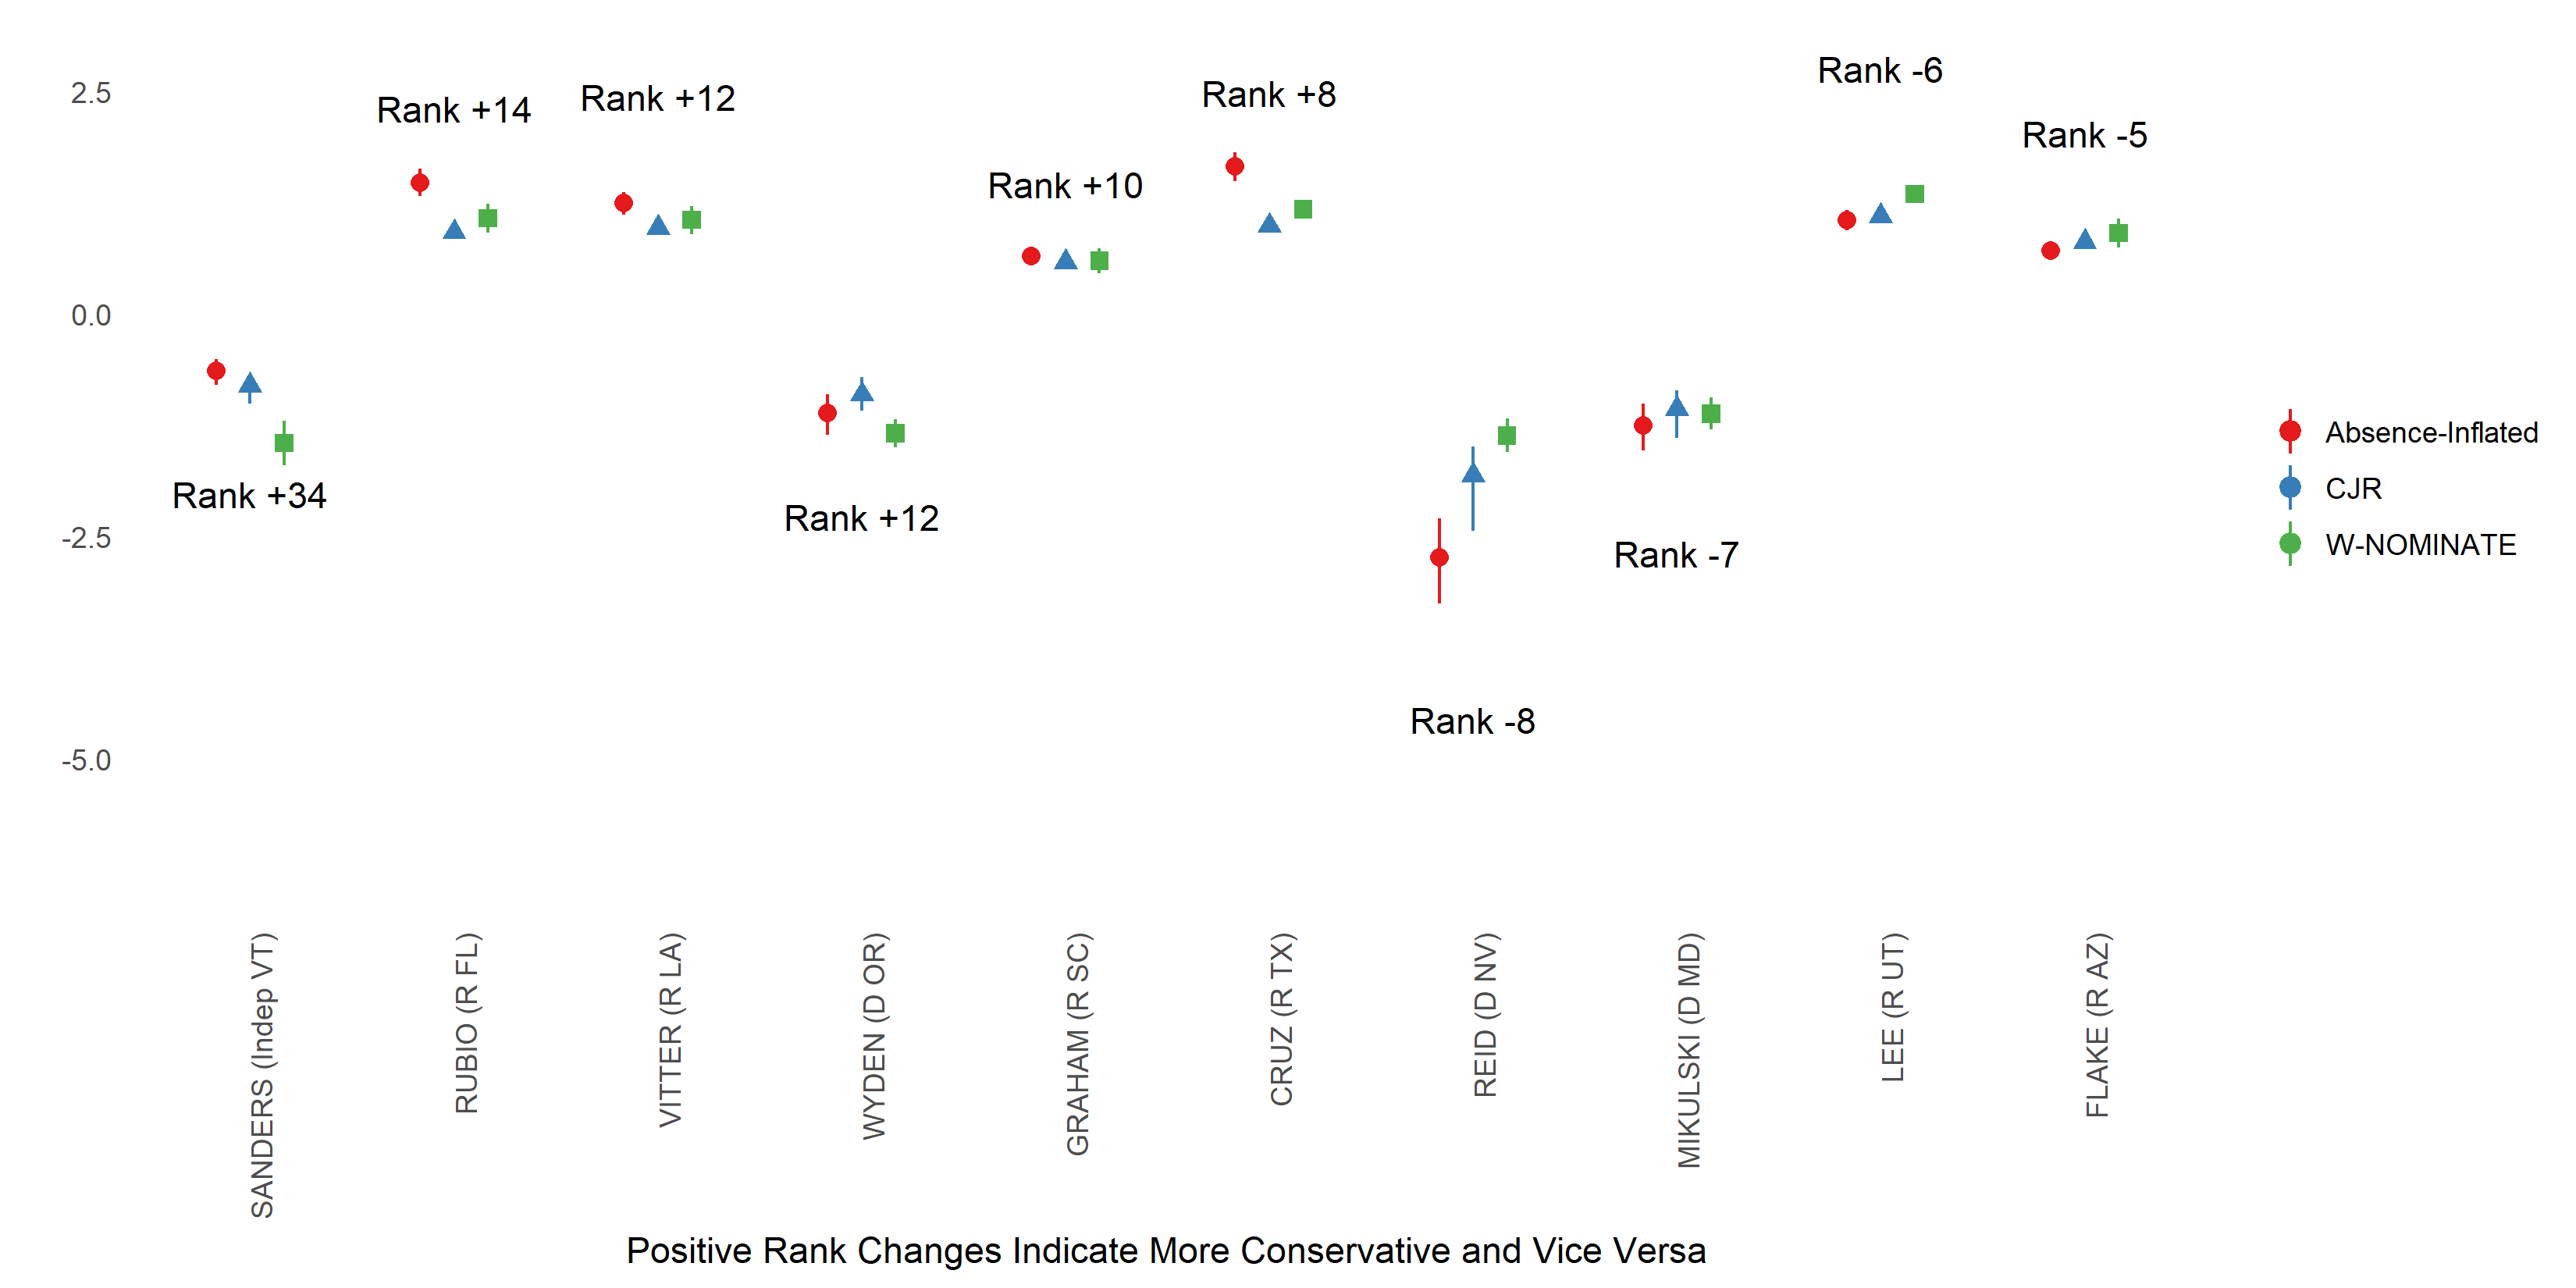
\includegraphics[width=0.8\linewidth]{big_diff}
	\end{figure}
	
	To track these changes within models, I show in Figure \ref{rank_sen} the largest changes in ranks between the absence-inflated model and the two standard models. Positive rank changes in the figure indicate a senator became more conservative as a result of having his or her absences included in the ideal point estimation. In some cases, such as with Bernie Sanders, the absence-inflated model is closer to the IRT-based CJR than the normal utility W-NOMINATE. But with Ted Cruz, Marco Rubio, and Harry Reid, who retired at the end of 114th Congress, the absence-inflated model is markedly different. With all three senators, the absence-inflated model shows the Congressmen moving towards the ideological extremes. This is likely because all three Congresspeople had an incentive to only show up to bills for which their absence points were relatively polarized: for Cruz and Rubio, pleasing the conservative base, and for Reid, a chance to live out his ideological principles with conviction before retirement.
	
	In addition, we can also analyze the bills that indicate that absences were particularly polarized by examining the $\gamma_j$ absence discrimination parameters. By looking at the highest (most conservative) and lowest (most liberal) values, we can find those absences which tend to divide legislators. Table \ref{con_bills} shows that liberal absences were most pronounced on a series of bills relating to climate change in early 2015. These strategic absences may be because of continuing American disagreement over climate change policy. Rather than have to adopt a conservative or liberal position on the issue, it would seem that at least some legislators sat out the votes. The bills with the highest conservative discrimination, shown in Table \ref{lib_bills}, do not indicate as much of a clear pattern, although there are several bills related to cyber security.
	
	\begin{table}[!h]
		\centering
		\caption{Bills With Highest Liberal Absence Discrimination}
		\label{con_bills}
		\begin{tabular}{p{6in}l}
			Description                                                                                                                                              & Date      \\
			\midrule
			To express the sense of Congress regarding climate change.                                                                                               & 1/22/2015 \\
			To express the sense of Congress regarding federally protected land.                                                                                     & 1/22/2015 \\
			To conform citizen suits under the Endangered Species Act of 1973.                                                                                       & 1/21/2015 \\
			To express the sense of Congress regarding climate change.                                                                                               & 1/21/2015 \\
			To express the sense of Congress regarding climate change.                                                                                               & 1/21/2015 \\
			To provide limits on the designation of new federally protected land.                                                                                    & 1/22/2015 \\
			To ensure that the storage and transportation of petroleum coke is regulated in a manner that ensures the protection of public and ecological health.    & 1/21/2015 \\
			To require the use of iron, steel, and manufactured goods produced in the United States in the construction of the Keystone XL Pipeline and facilities.  & 1/20/2015 \\
			To express the sense of the Senate that climate change is real and not a hoax.                                                                           & 1/21/2015 \\
			To ensure that oil transported through the Keystone XL pipeline into the United States is used to reduce United States dependence on Middle Eastern oil. & 1/20/2015
		\end{tabular}
	\end{table}

\begin{table}[h!]
	\centering
	\caption{Bills With Highest Conservative Absence Discrimination}
	\label{lib_bills}
	\begin{tabular}{p{6in}l}
		Description                                                                                                                                                                                                                              & Date       \\
		\midrule
		To limit the availability of amounts authorized to be appropriated for overseas contingency operations pending relief from the spending limits under the Budget Control Act of 2011.                                                     & 6/9/2015   \\
		To improve the requirements relating to removal of personal information from cyber threat indicators before sharing.                                                                                                                     & 10/27/2015 \\
		To strike the FOIA exemption.                                                                                                                                                                                                            & 10/27/2015 \\
		To protect information that is reasonably believed to be personal information or information that identifies a specific person.                                                                                                          & 10/27/2015 \\
		To strengthen the Justice for Victims of Trafficking Act by incorporating additional bipartisan amendments.                                                                                                                              & 4/22/2015  \\
		To improve the bill.                                                                                                                                                                                                                     & 4/22/2015  \\
		An original concurrent resolution setting forth the congressional budget for the United States Government for fiscal year 2016 and setting forth the appropriate budgetary levels for fiscal years 2017 through 2025.                    & 4/15/2015  \\
		To exempt from the capability and process within the Department of Homeland Security communication between a private entity and the Federal Bureau of Investigation or the United States Secret Service regarding cybersecurity threats. & 10/27/2015 \\
		To improve the definitions of cybersecurity threat and cyber threat indicator.                                                                                                                                                           & 10/27/2015 \\
		An original bill to improve cybersecurity in the United States through enhanced sharing of information about cybersecurity threats, and for other purposes.                                                                              & 10/27/2015
	\end{tabular}
\end{table}

To analyze these bills, it is possible to plot the bill midpoints against the ideal point distribution and see which legislators are choosing to be absent on these particular bills. I selected the bill with the second-highest absence discrimination among conservatives, which was the 2015 Cybersecurity Information Sharing Act that was sponsored by Richard Burr, a Republican from North Carolina. The bill mid-points for the non-inflated and inflated (absence) parameters are shown in Figure \ref{cyber} along with rug lines indicating the 10\%-90\% HPD interval. The senators who chose not to show up for this bill, which would have allowed corporations to turn over data to the federal government for the purposes of fighting cybercrimes, include Ted Cruz, Marco Rubio, Rand Paul and David Vitter. The vote occurred in late October, which would explain why Cruz, Rubio and Paul would have had a reason to be absent, but does not explain why they chose not to show up for a vote on this particular bill. The bill caused some controversy among people who feared the federal government gaining access to their data via a back-door \parencite{cisa2015}, and it seems plausible that the senators on the campaign trail would have wanted to avoid making a strong statement against or for the bill. As can be seen in the figure, the Republican party itself was remarkably split on this bill, with both moderate and conservative senators voting for it. The model cannot explain the full story behind this bill, of course, but it does serve to highlight those bills in which absences are particularly noticeable and worthy of further analysis.

\begin{figure}
	\caption{Bill Midpoints for Cybersecurity Information Sharing Act}\label{cyber}
	\centering
	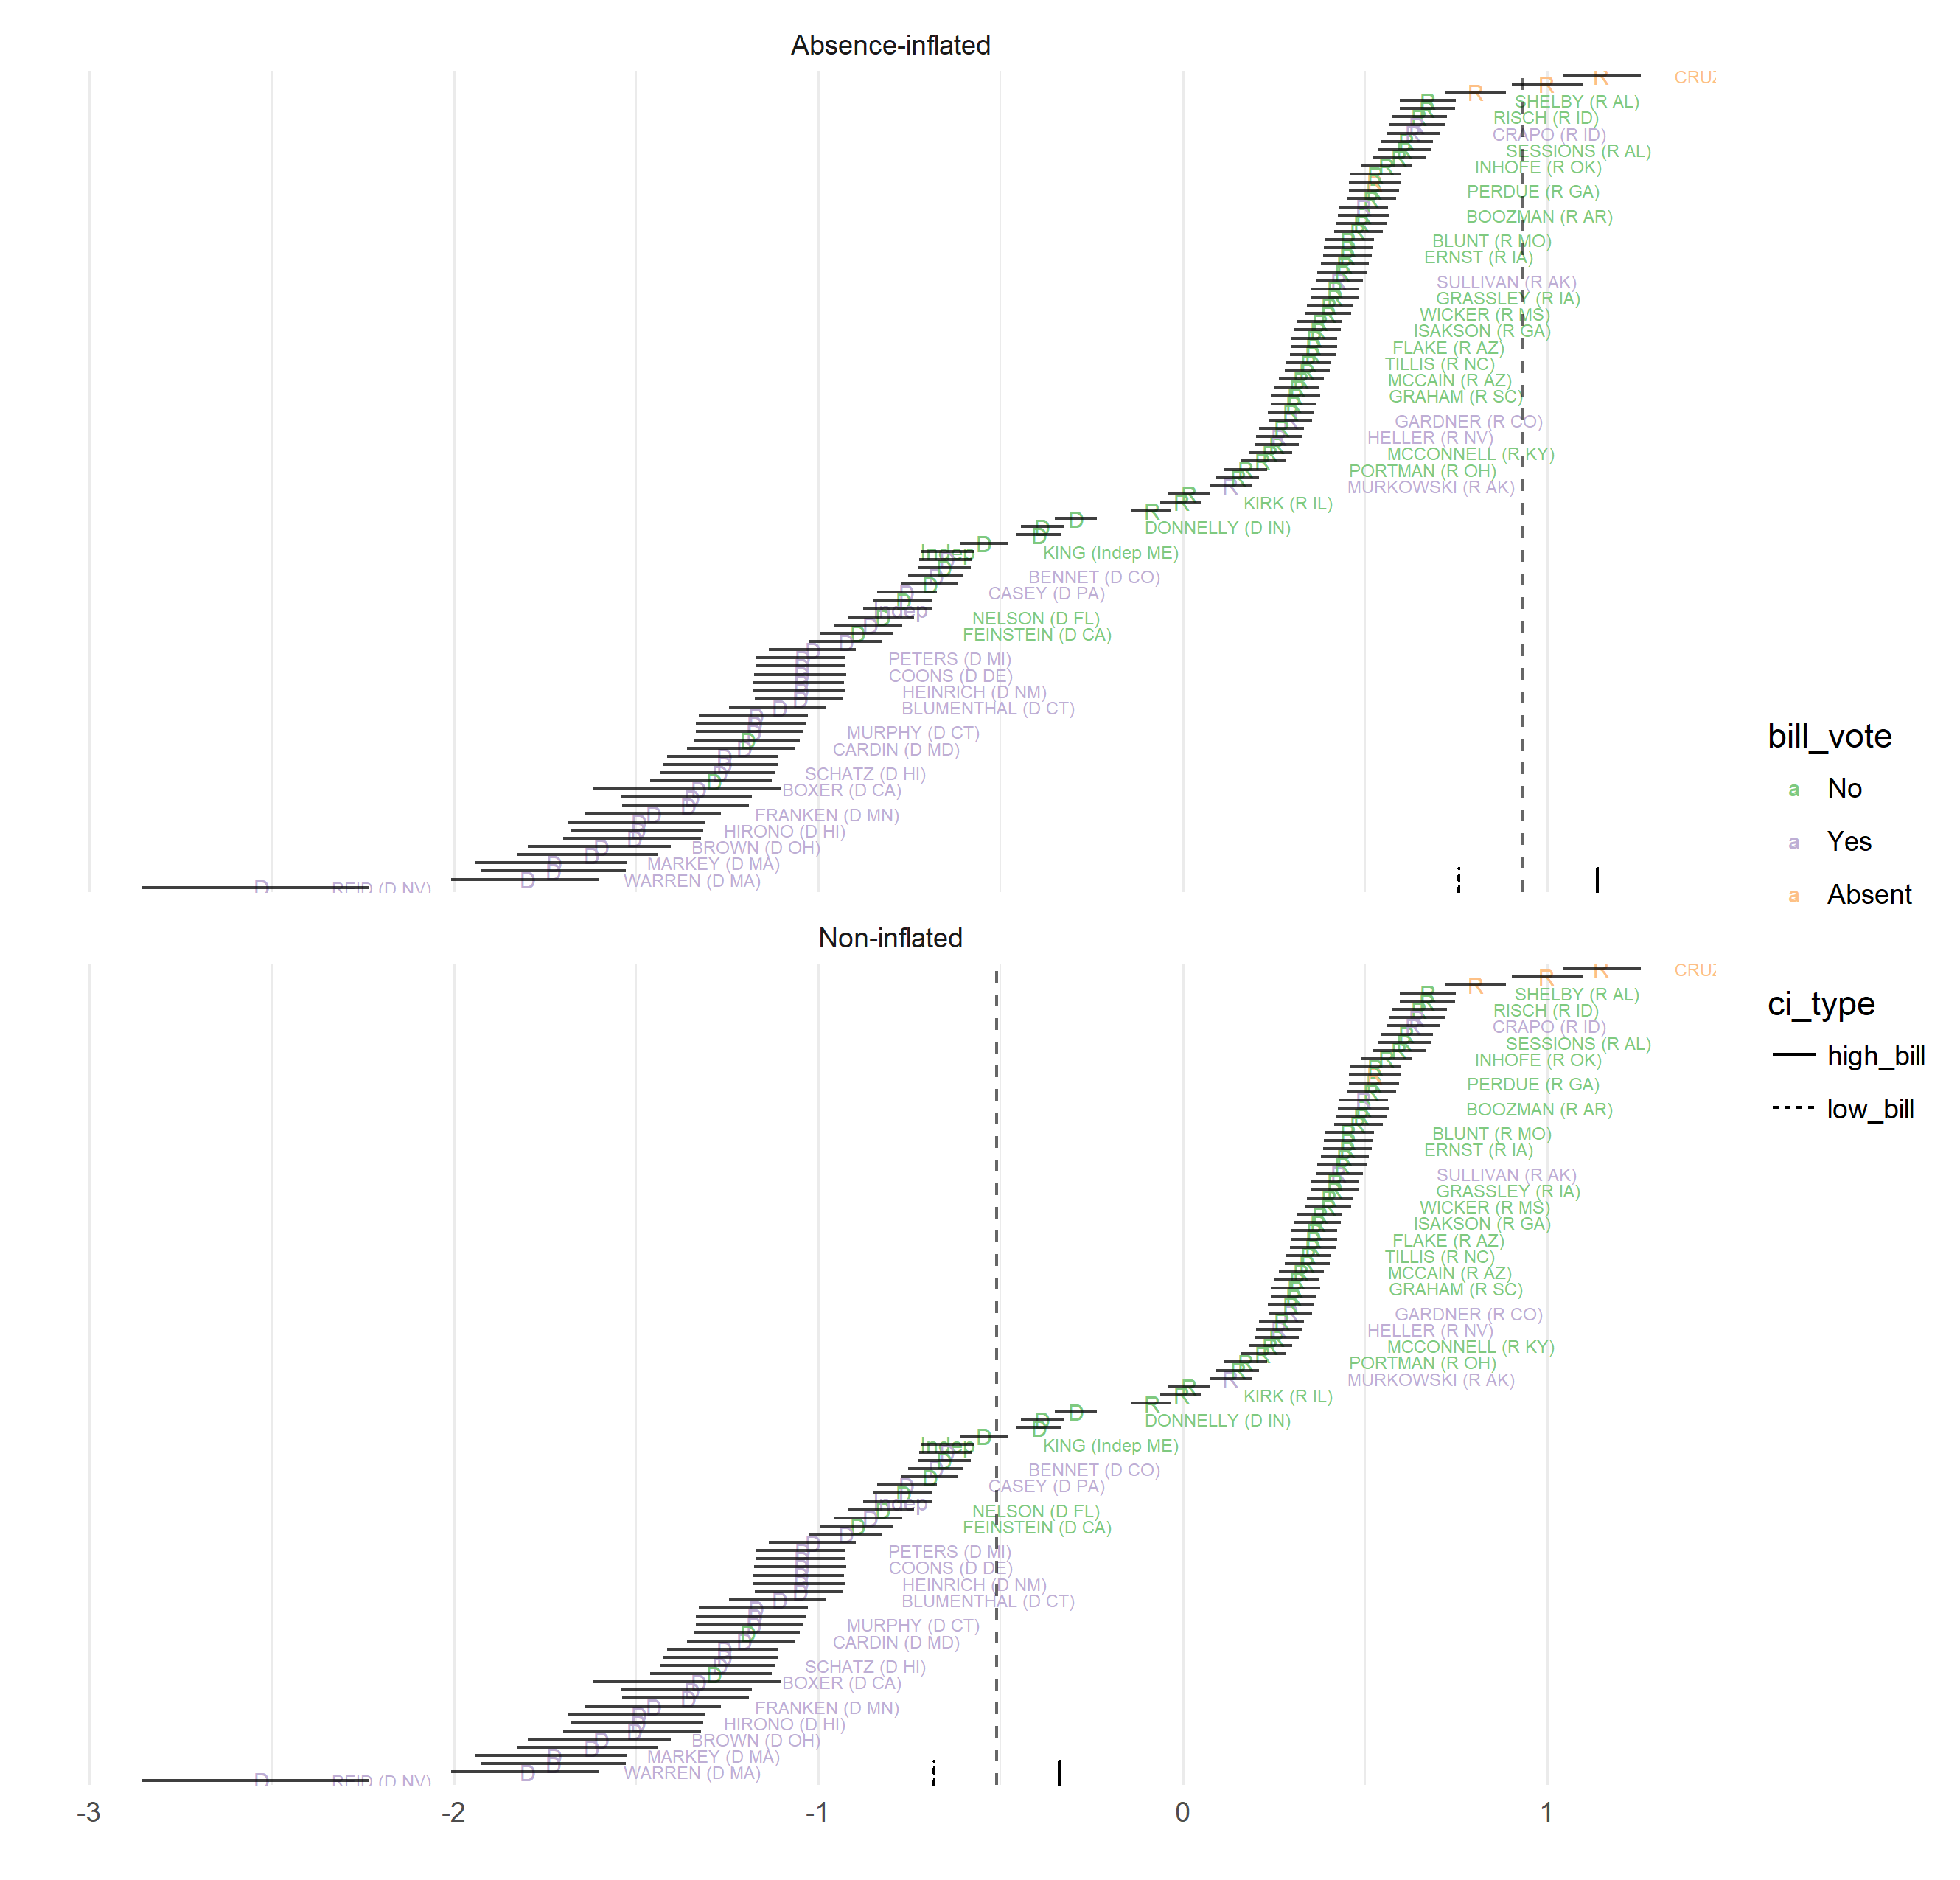
\includegraphics[width=\linewidth]{con_discrim_bill}
\end{figure}

In addition to substantive evaluation of the models, I also use predictive criteria to compare the absence-inflated IRT versus the standard approaches. Figures \ref{fpr_cjr} and \ref{fpr_wnom} compare false-positive rates (false positives divided by total number of true positives) and Figures \ref{fnr_cjr} and \ref{fnr_wnom} compare false-negative rates (false negatives divided by total number of true negatives). A false positive means that the model predicted that a legislator would vote for a bill when in fact they did not, while a false negative means that a model predicted that a legislator would vote against a bill when in fact they did not. Each plot also includes the overall mean false positive/negative rate as a vertical line. These statistics were calculated on the number of bills analyzed by W-NOMINATE in order to make them comparable across models because W-NOMINATE drops bills that have unanimous votes. 
\begin{figure}[h!]
	\caption{Comparison of False Positive Rates for CJR vs. Absence-Inflated}\label{fpr_cjr}
	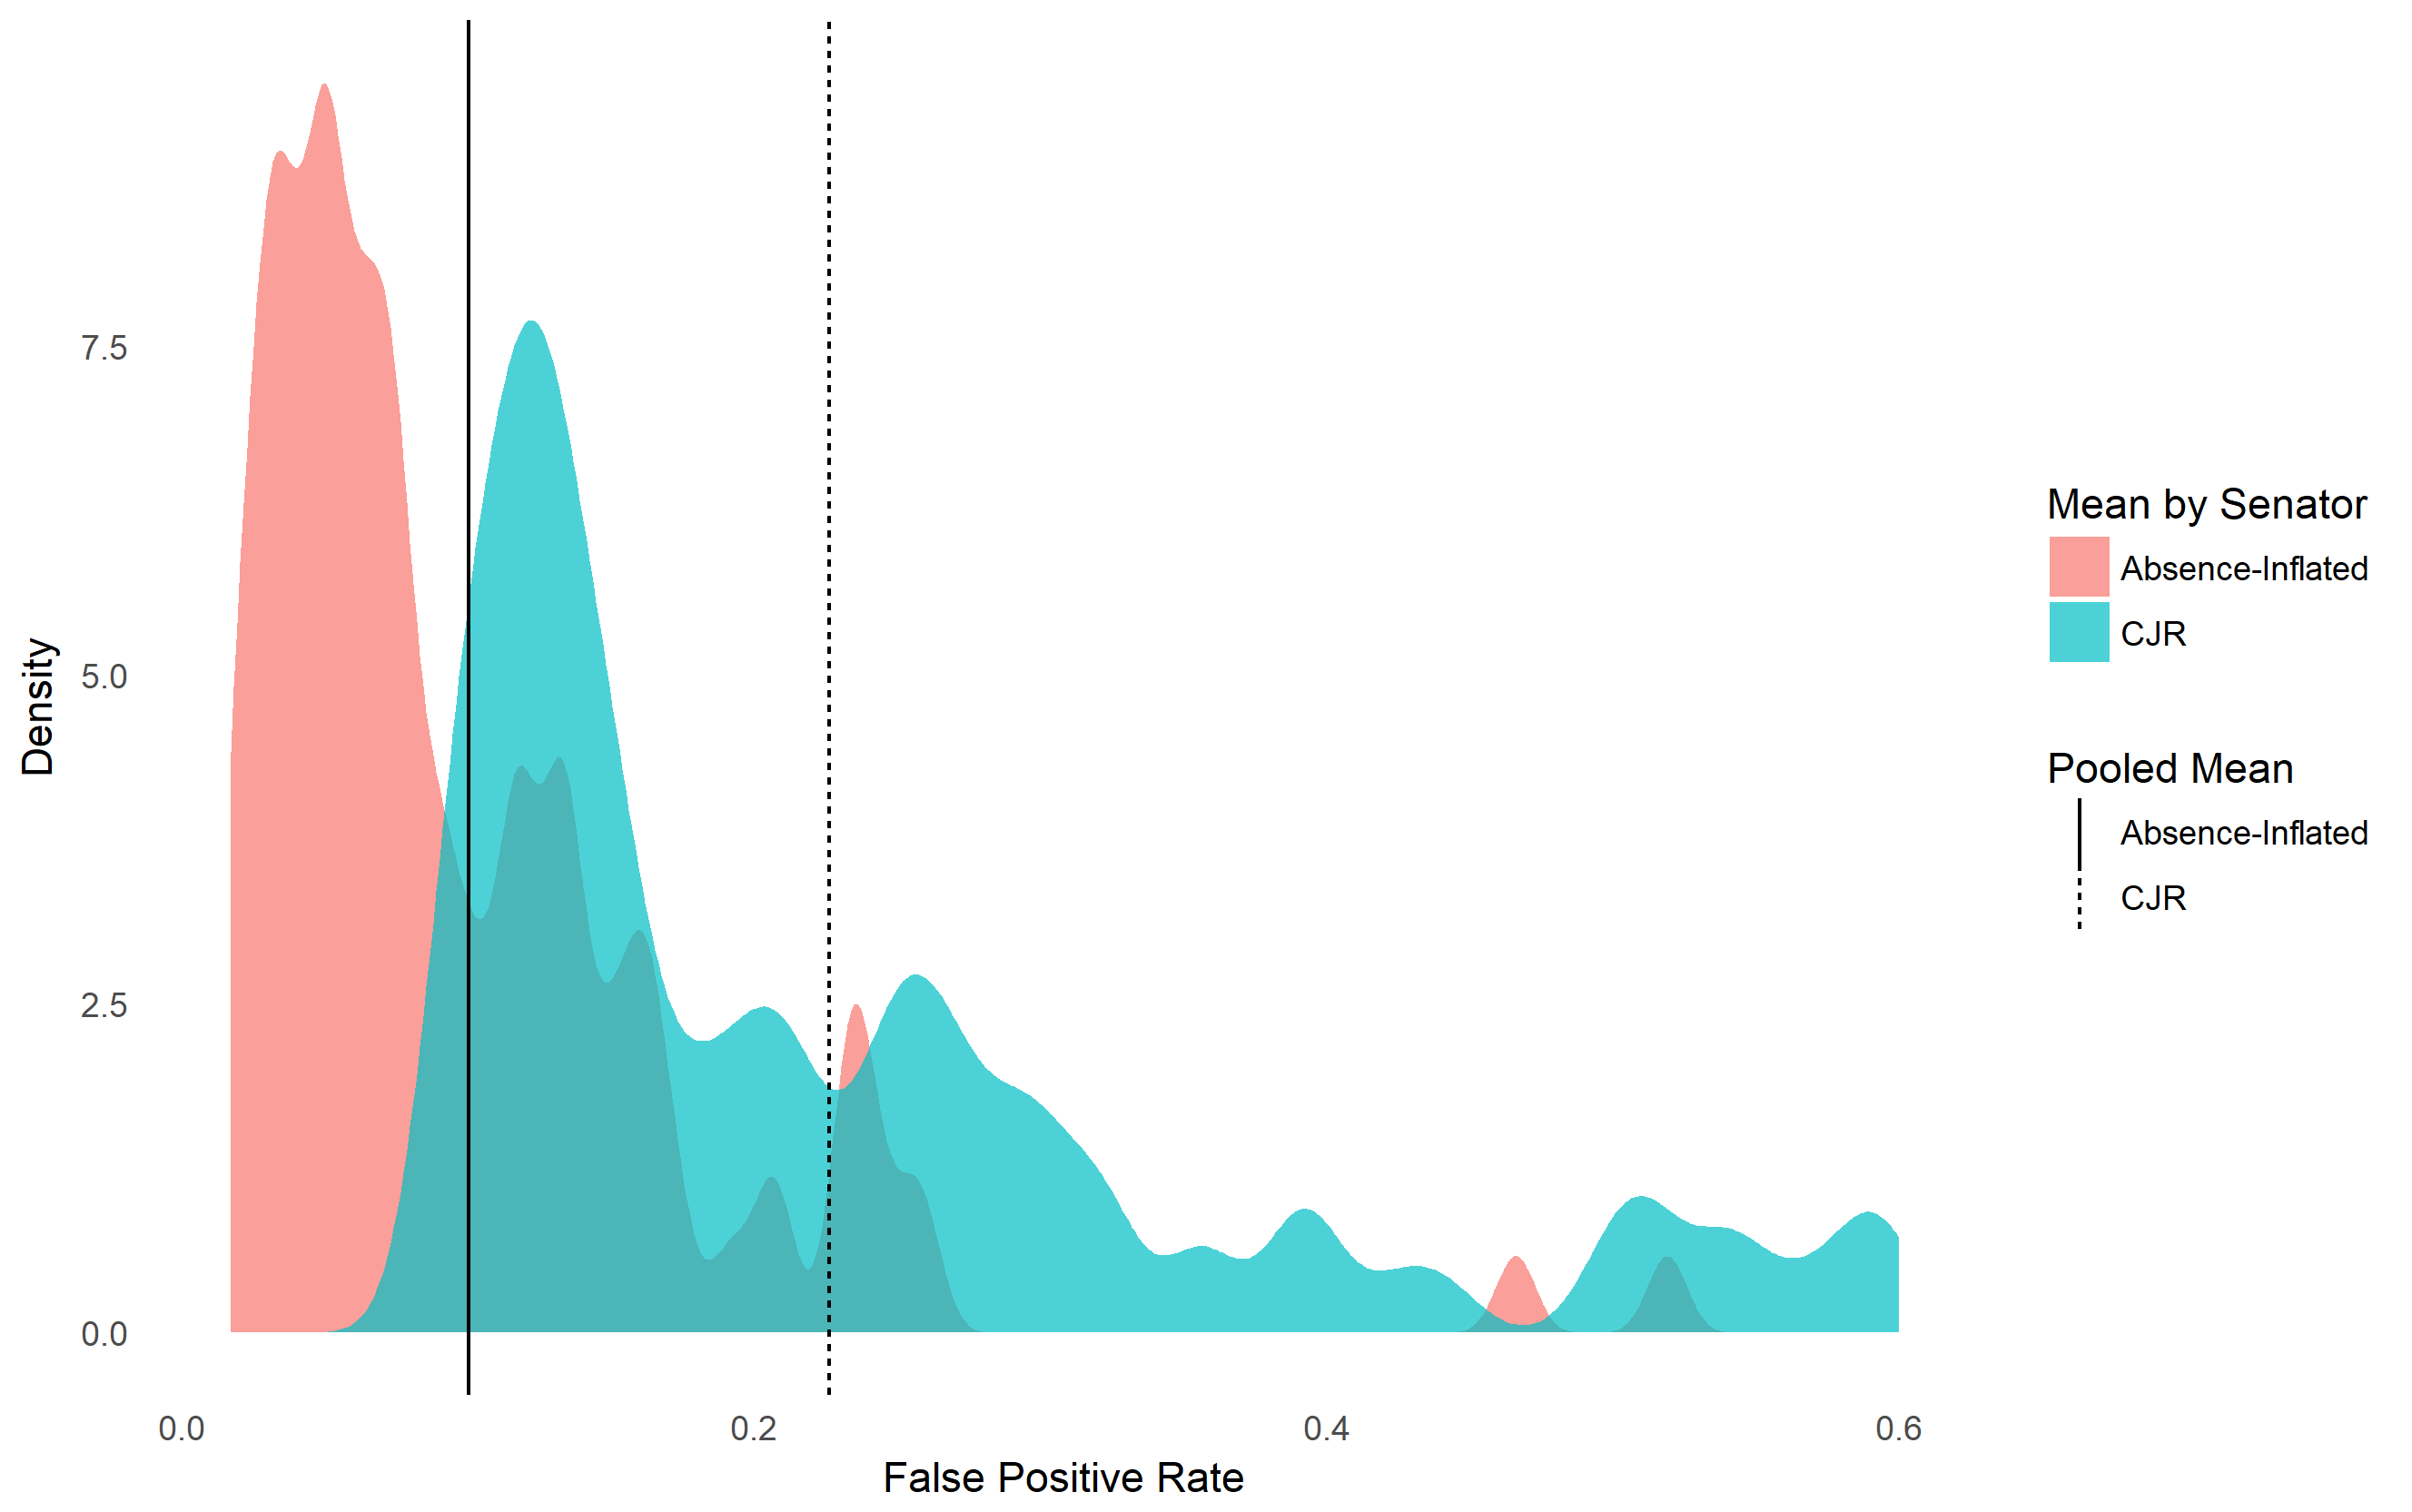
\includegraphics[width=0.9\linewidth]{false_positive_CJR_sen}
\end{figure}
\begin{figure}[h!]
	\caption{Comparison of False Negative Rates for CJR vs. Absence-Inflated}\label{fnr_cjr}
		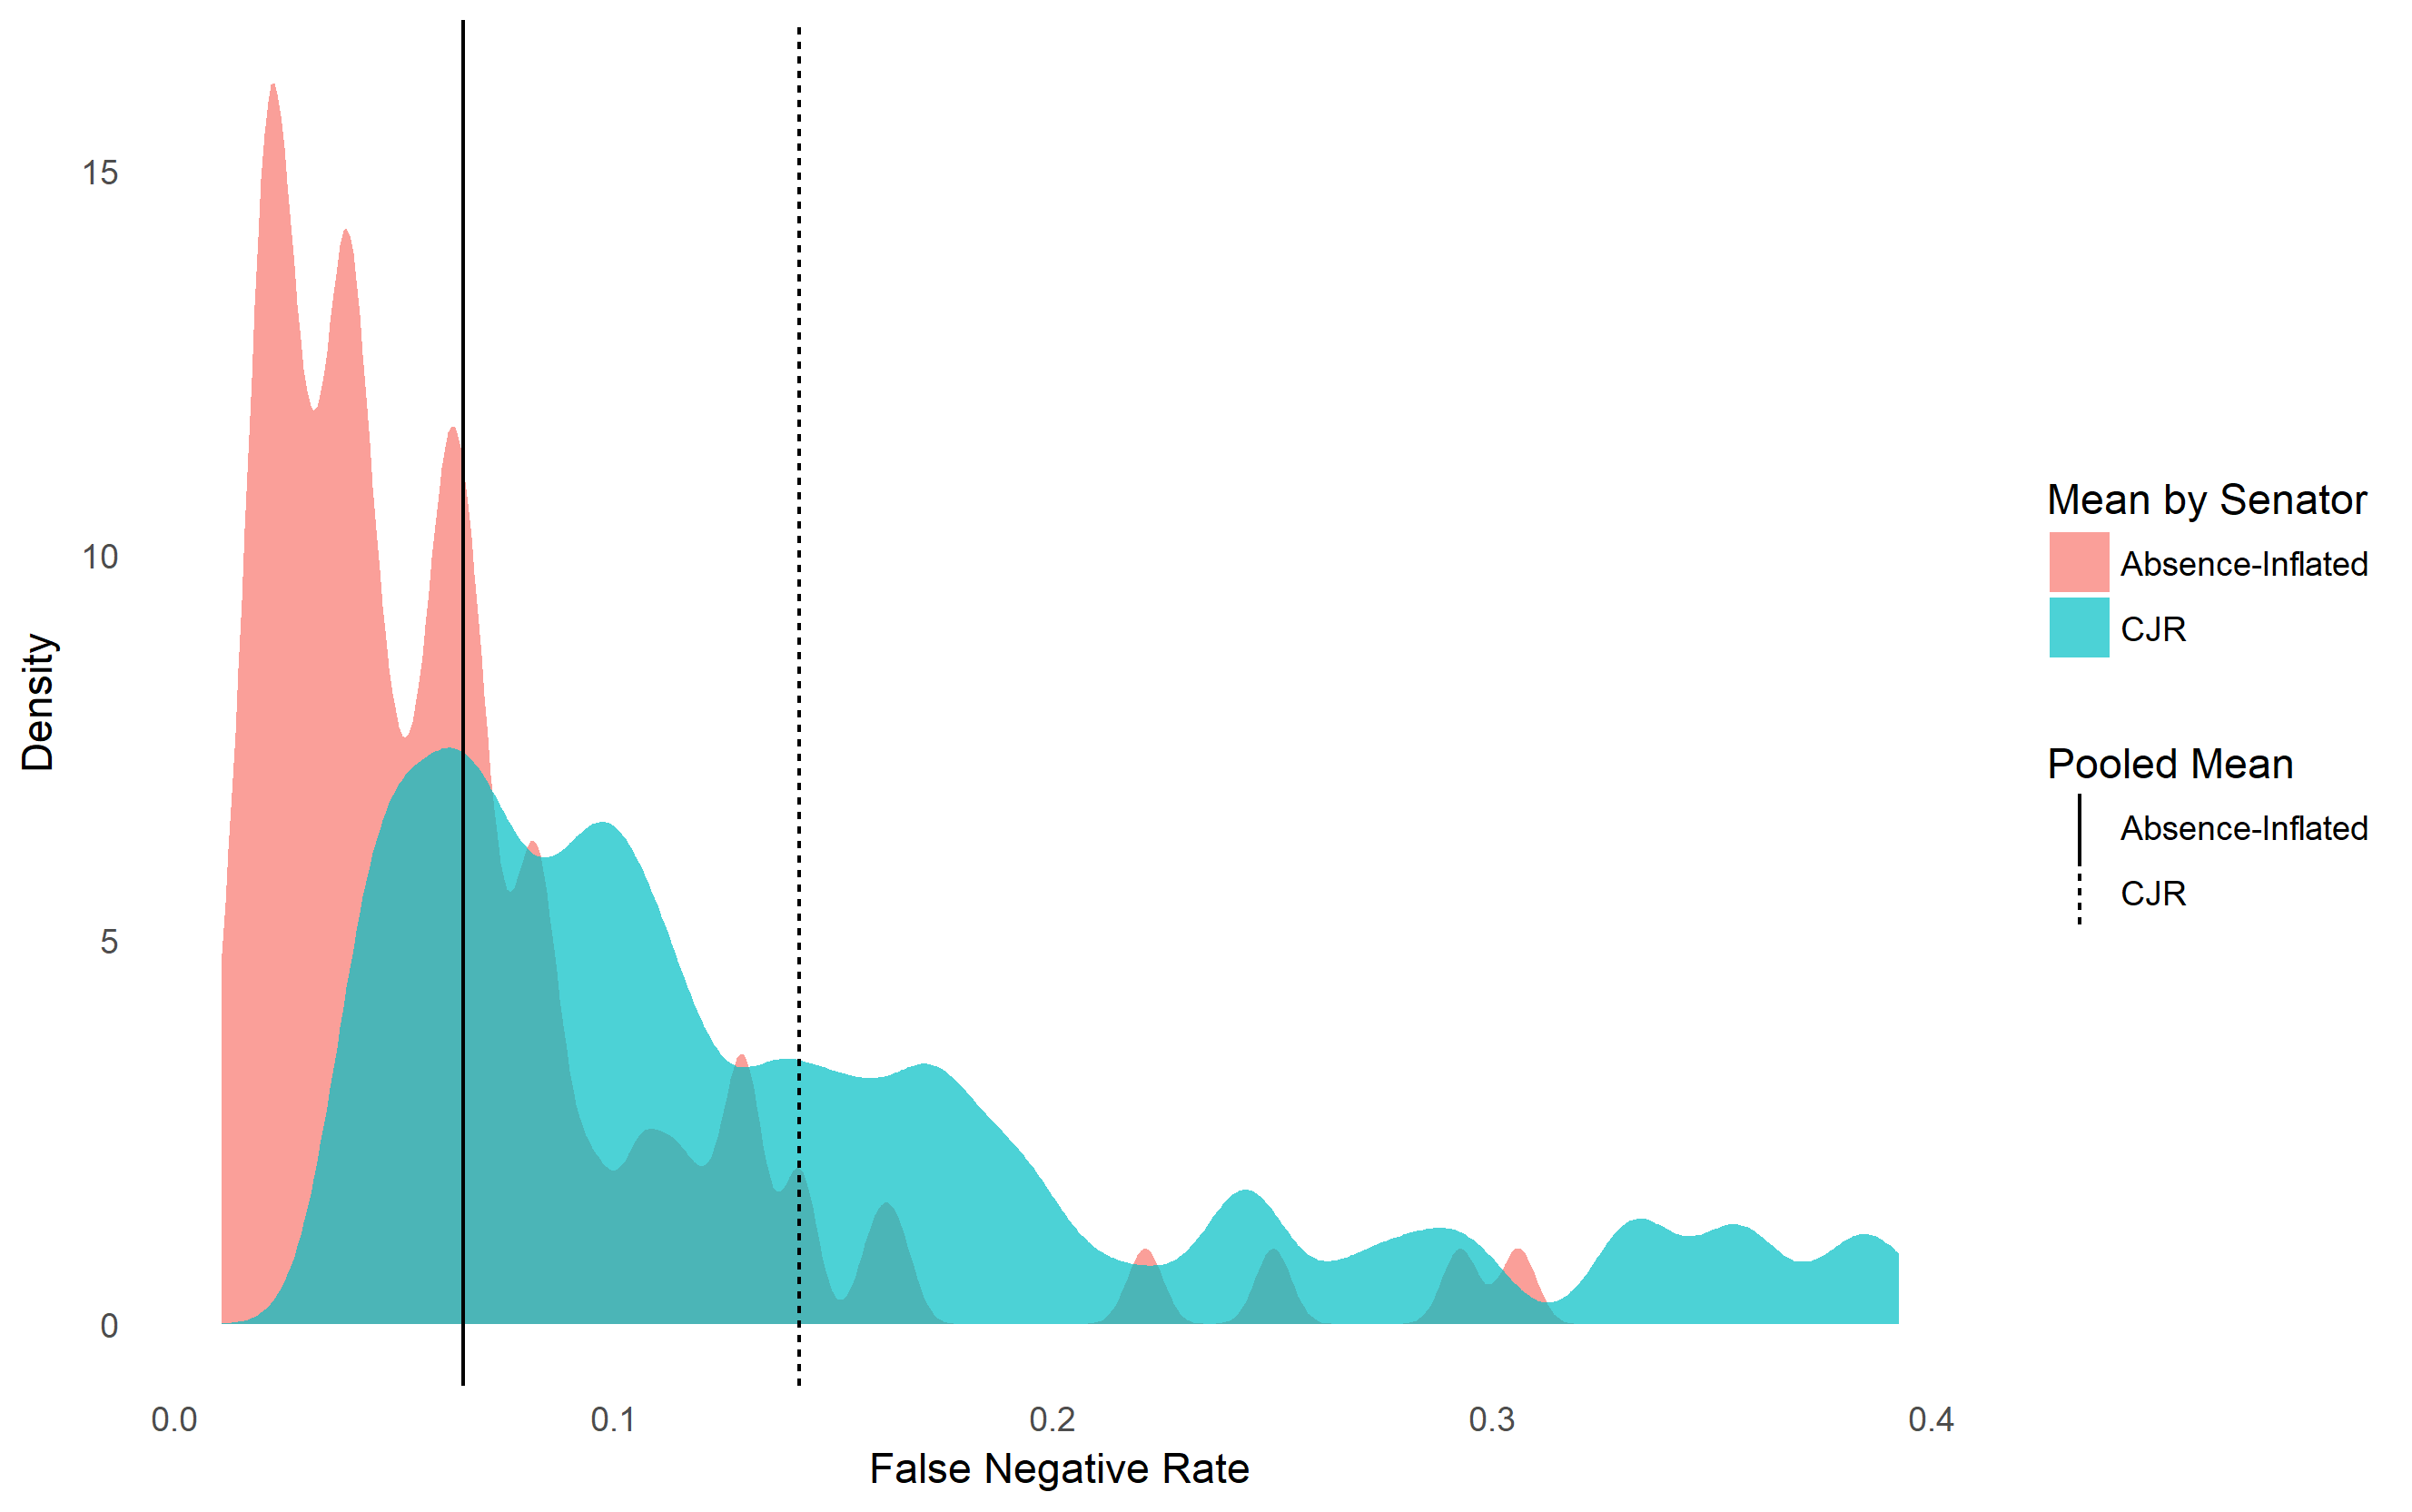
\includegraphics[width=0.9\linewidth]{false_negative_CJR_sen}
\end{figure}
\begin{figure}[h!]
	\caption{Comparison of False Positive Rates for W-NOMINATE vs. Absence-Inflated}\label{fpr_wnom}
		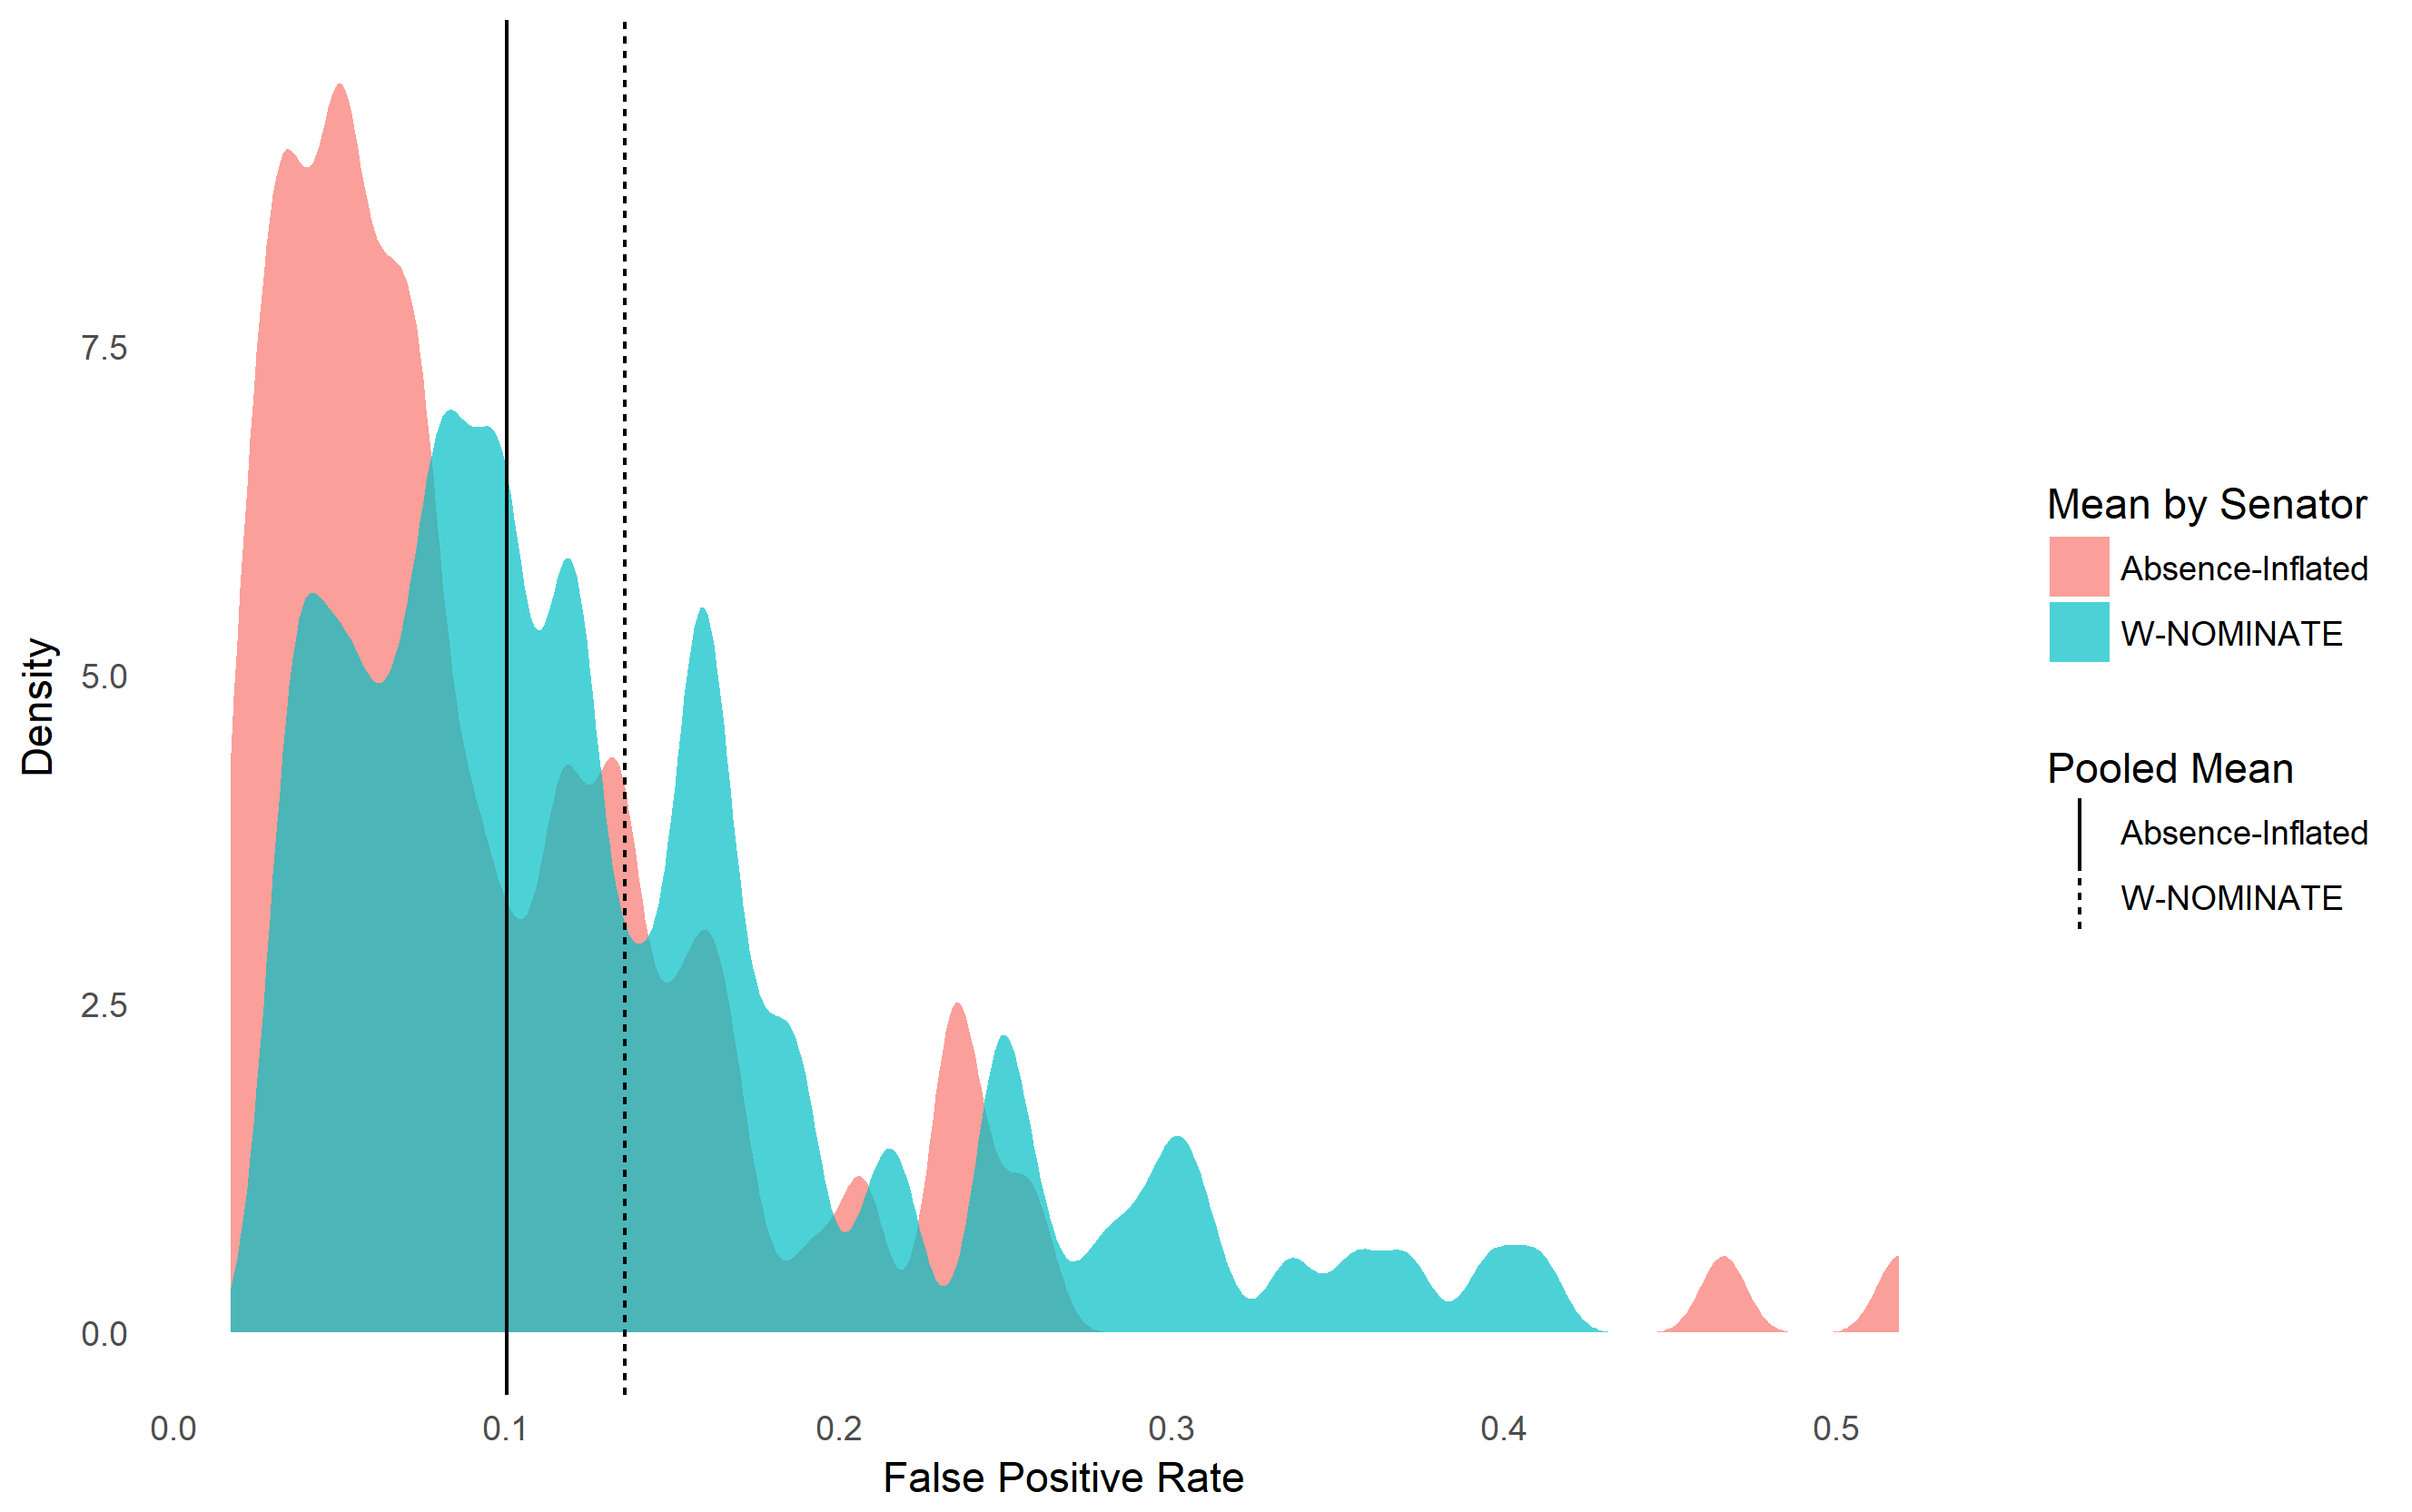
\includegraphics[width=0.9\linewidth]{false_positive_WN_sen}
\end{figure}
\begin{figure}[h!]
	\caption{Comparison of False Negative Rates for W-NOMINATE vs. Absence-Inflated}\label{fnr_wnom}
			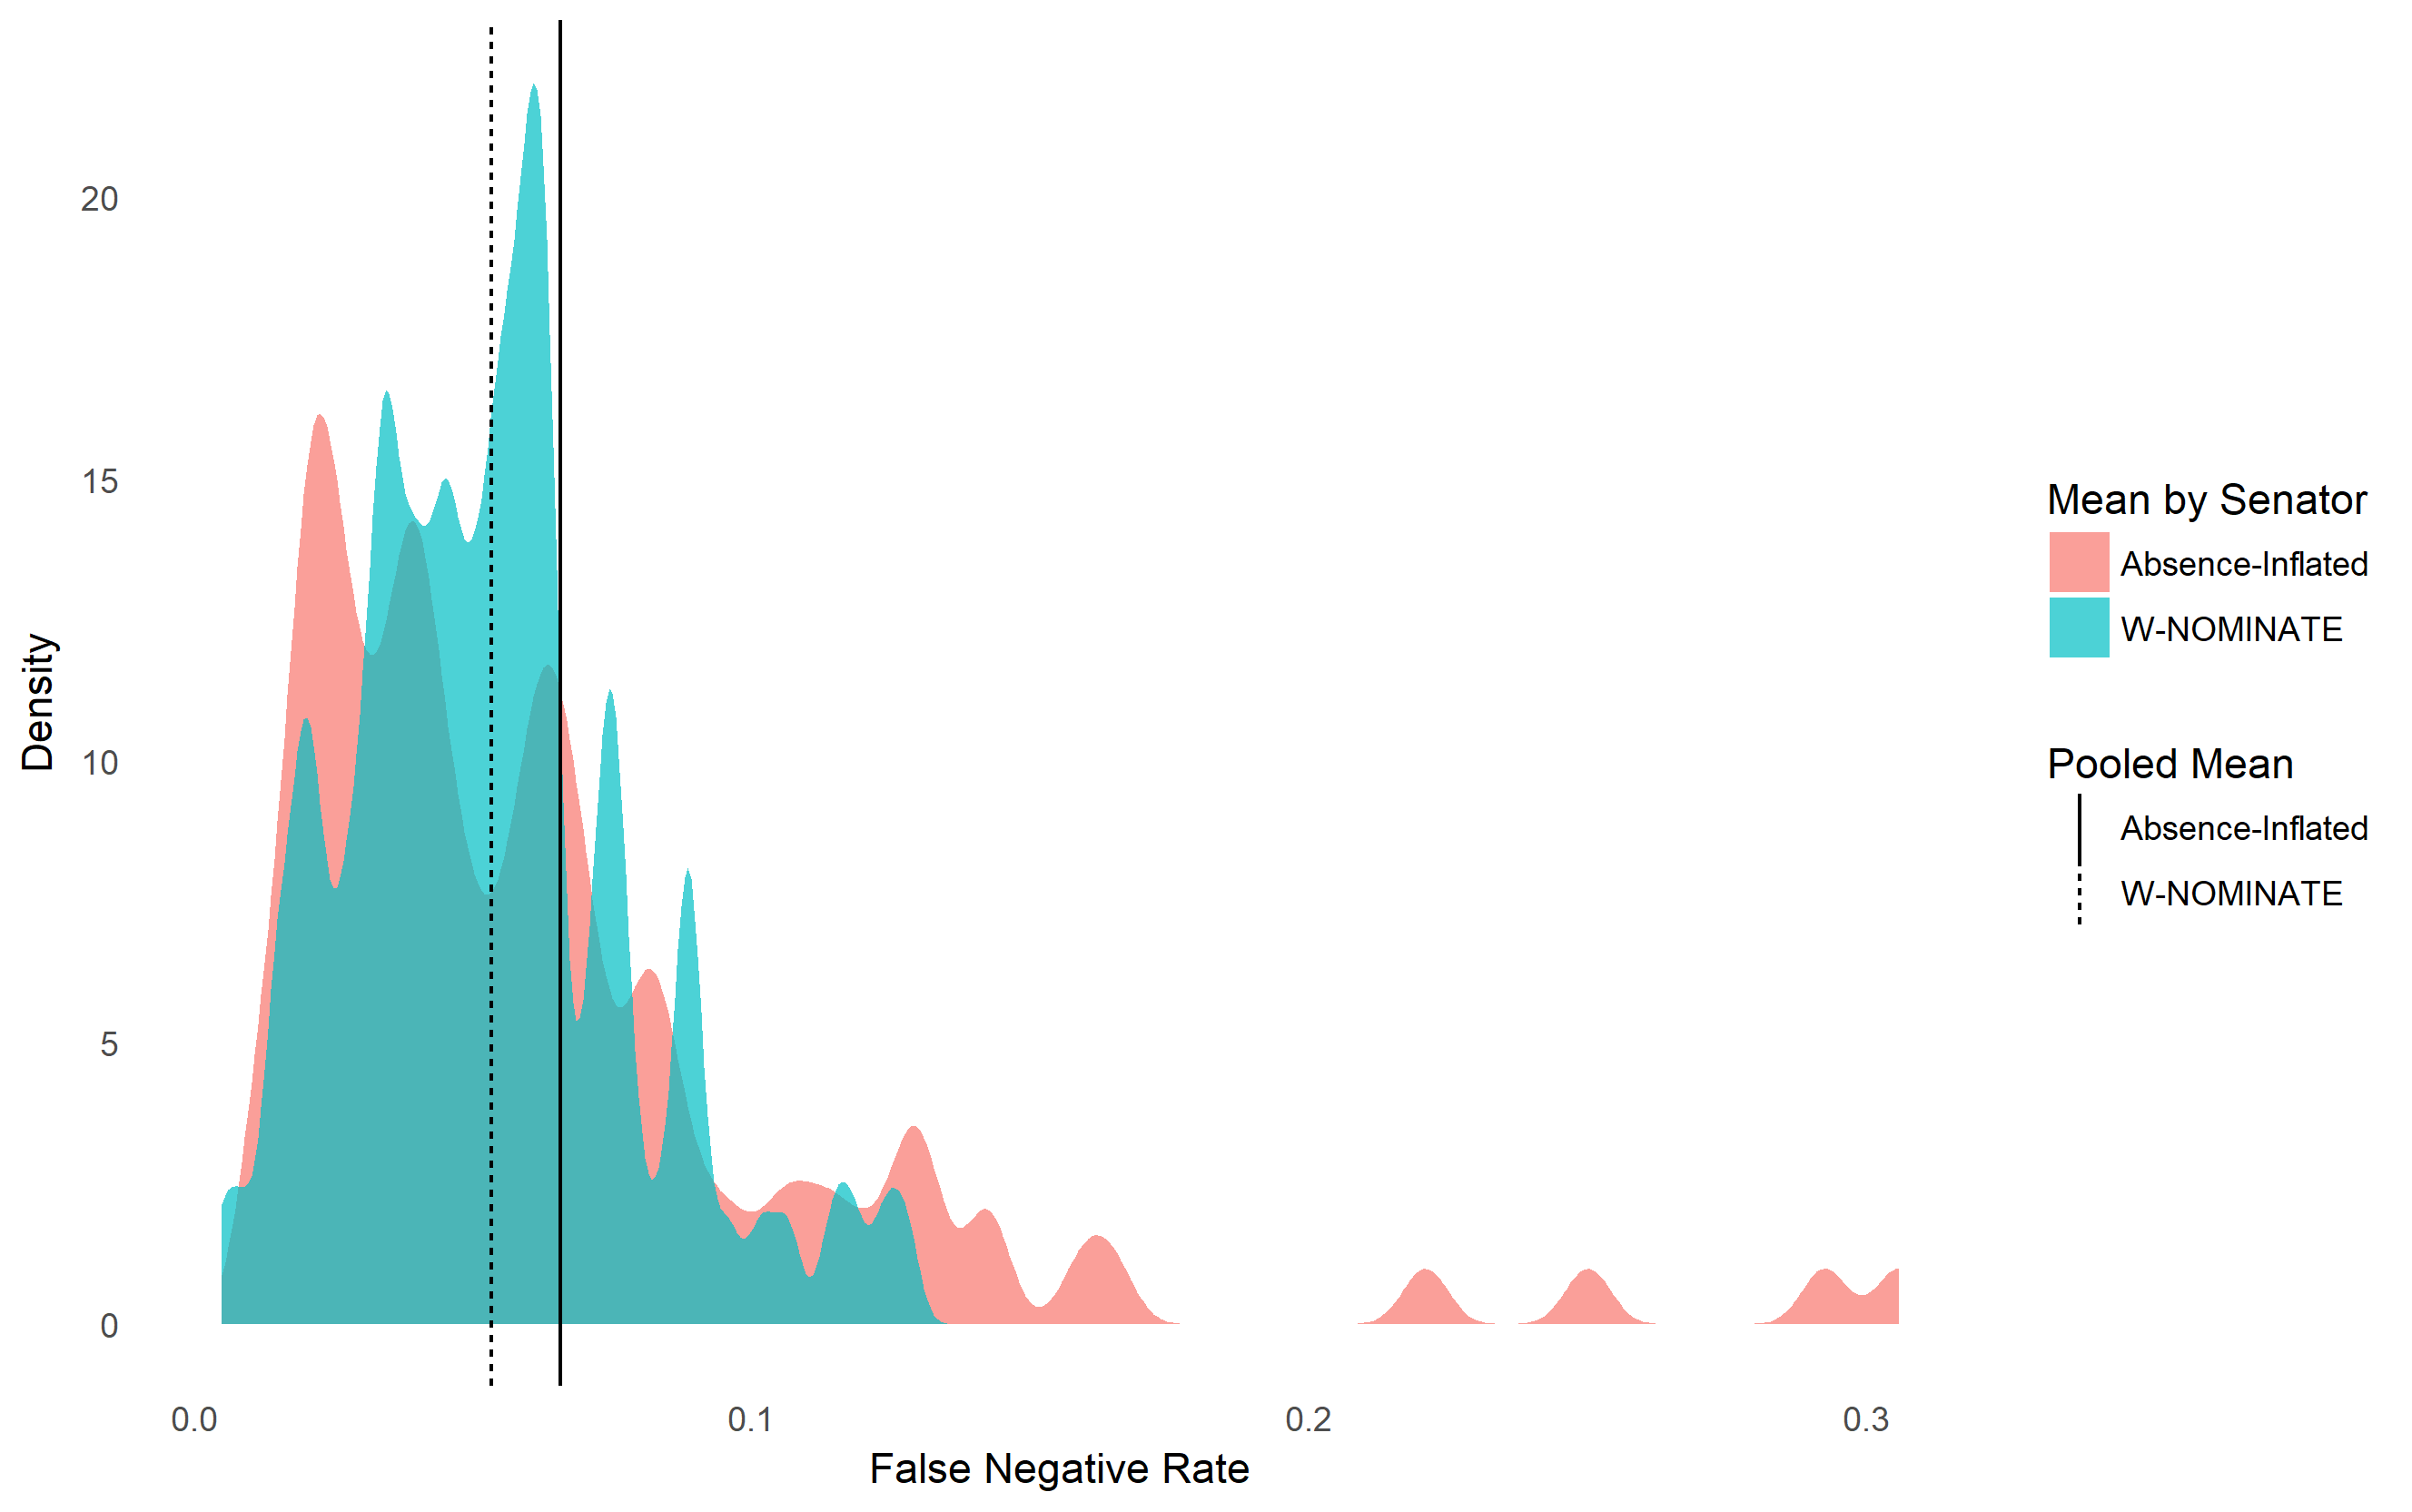
\includegraphics[width=0.9\linewidth]{false_negative_WN_sen}
\end{figure}

What the figures show is that, generally speaking, the absence-inflated model has better predictive performance compared to CJR and W-NOMINATE, except for W-NOMINATE's false negative rates, which are slightly lower than the absence-inflated model. This latter result is primarily driven by a handful of legislators, including Bernie Sanders, who have very high false negative rates. What is also interesting to note is that W-NOMINATE has much lower false positive and false negative rates than CJR even though the ideal points estimated by the models are highly correlated. The exact reasons for this discrepancy are unclear, and have not been noted before in the literature comparing these models \parencite{carroll2009,jackman2004,carroll2013}. One plausible explanation is the more complicated Gaussian utility function embedded in the W-NOMINATE model, which could provide a closer fit to the data and also account for its strong performance in the mixture model framework of \textcite{carroll2013}. Finally, it is interesting to note that both CJR and W-NOMINATE tend to perform better at minimizing false negative rates, or Type II errors, rather than false positive rates, or Type I errors. The absence-inflated model also shows better aptitude at minimizing false negative rates, although the difference is not as strongly pronounced.

While predictive performance is not the primary criterion for evaluating ideal point models as the quantity of interest is the unobserved ideal points, the results presented suggest that the absence-inflated model is able to capitalize on strategic information about ideal points encoded in absences to lower the rate of miscoded votes, in particular yes votes, and in some cases no votes as well. What is important to note is that these statistics were only calculated on the subset of the data of divided roll-call votes in which yes and no votes capture the majority of the information, so it was a more difficult test for the absence-inflated model to pass. 




	
	\subsection*{Tunisian Parliament}
	
	The Tunisian Assembly of Representatives is a legislative body that held its first free and fair elections in the fall of 2014 after the fall of Zine Abedine Ben Ali's dictatorship in 2011. As is the case in many transitional democracies, parliamentary blocs tend to be more fluid and idealogical positions on policy issues are relatively unknown. In addition, the 2014 parliament witnessed the election of many MPs who had outside businesses to run and other conflicts with showing up to the chamber, which led to very high absence rates, sometimes as high as 50 percent. The dataset here presented was obtained from a Tunisian NGO and shows the full voting record, including votes on amendments, in the parliament from 2014 up to the summer of 2016. 
	
	Figure \ref{tunis_arp_hist} shows the histogram of votes for this dataset, revealing the important differences between a transitional democracy and a well-established democracy like the US Congress. Absences are the single most common recorded category of votes in the parliament. In addition, there are far more yes votes than no votes, which is a result of an over-sized parliamentary coalition. In Tunisia, the two largest parties, the secular Nidaa Tounes and the Islamist Nahda, joined together in a unity coalition out of a concern that democratic competition was de-stabilizing the country. Consequently, more than two-thirds of the MPs are at least nominally affiliated with the government, leaving little room for opposition. As a result, MPs tend to express their disagreement through abstentions and/or absences, a phenomenon that has been noted as a common occurrence in parliamentary coalitions with strong control over how MPs vote \parencite{brauninger2016}. However, because standard ideal point models tend to drop both absences and abstentions, these models will tend to show the governing coalition as a monolith because most MPs can only use abstentions or absences to register their disagreement or disapproval of their coalition's policies. 
	
	\begin{figure}
		\centering
		\caption{Vote Histogram of Tunisian Assembly of Representatives}\label{tunis_arp_hist}
		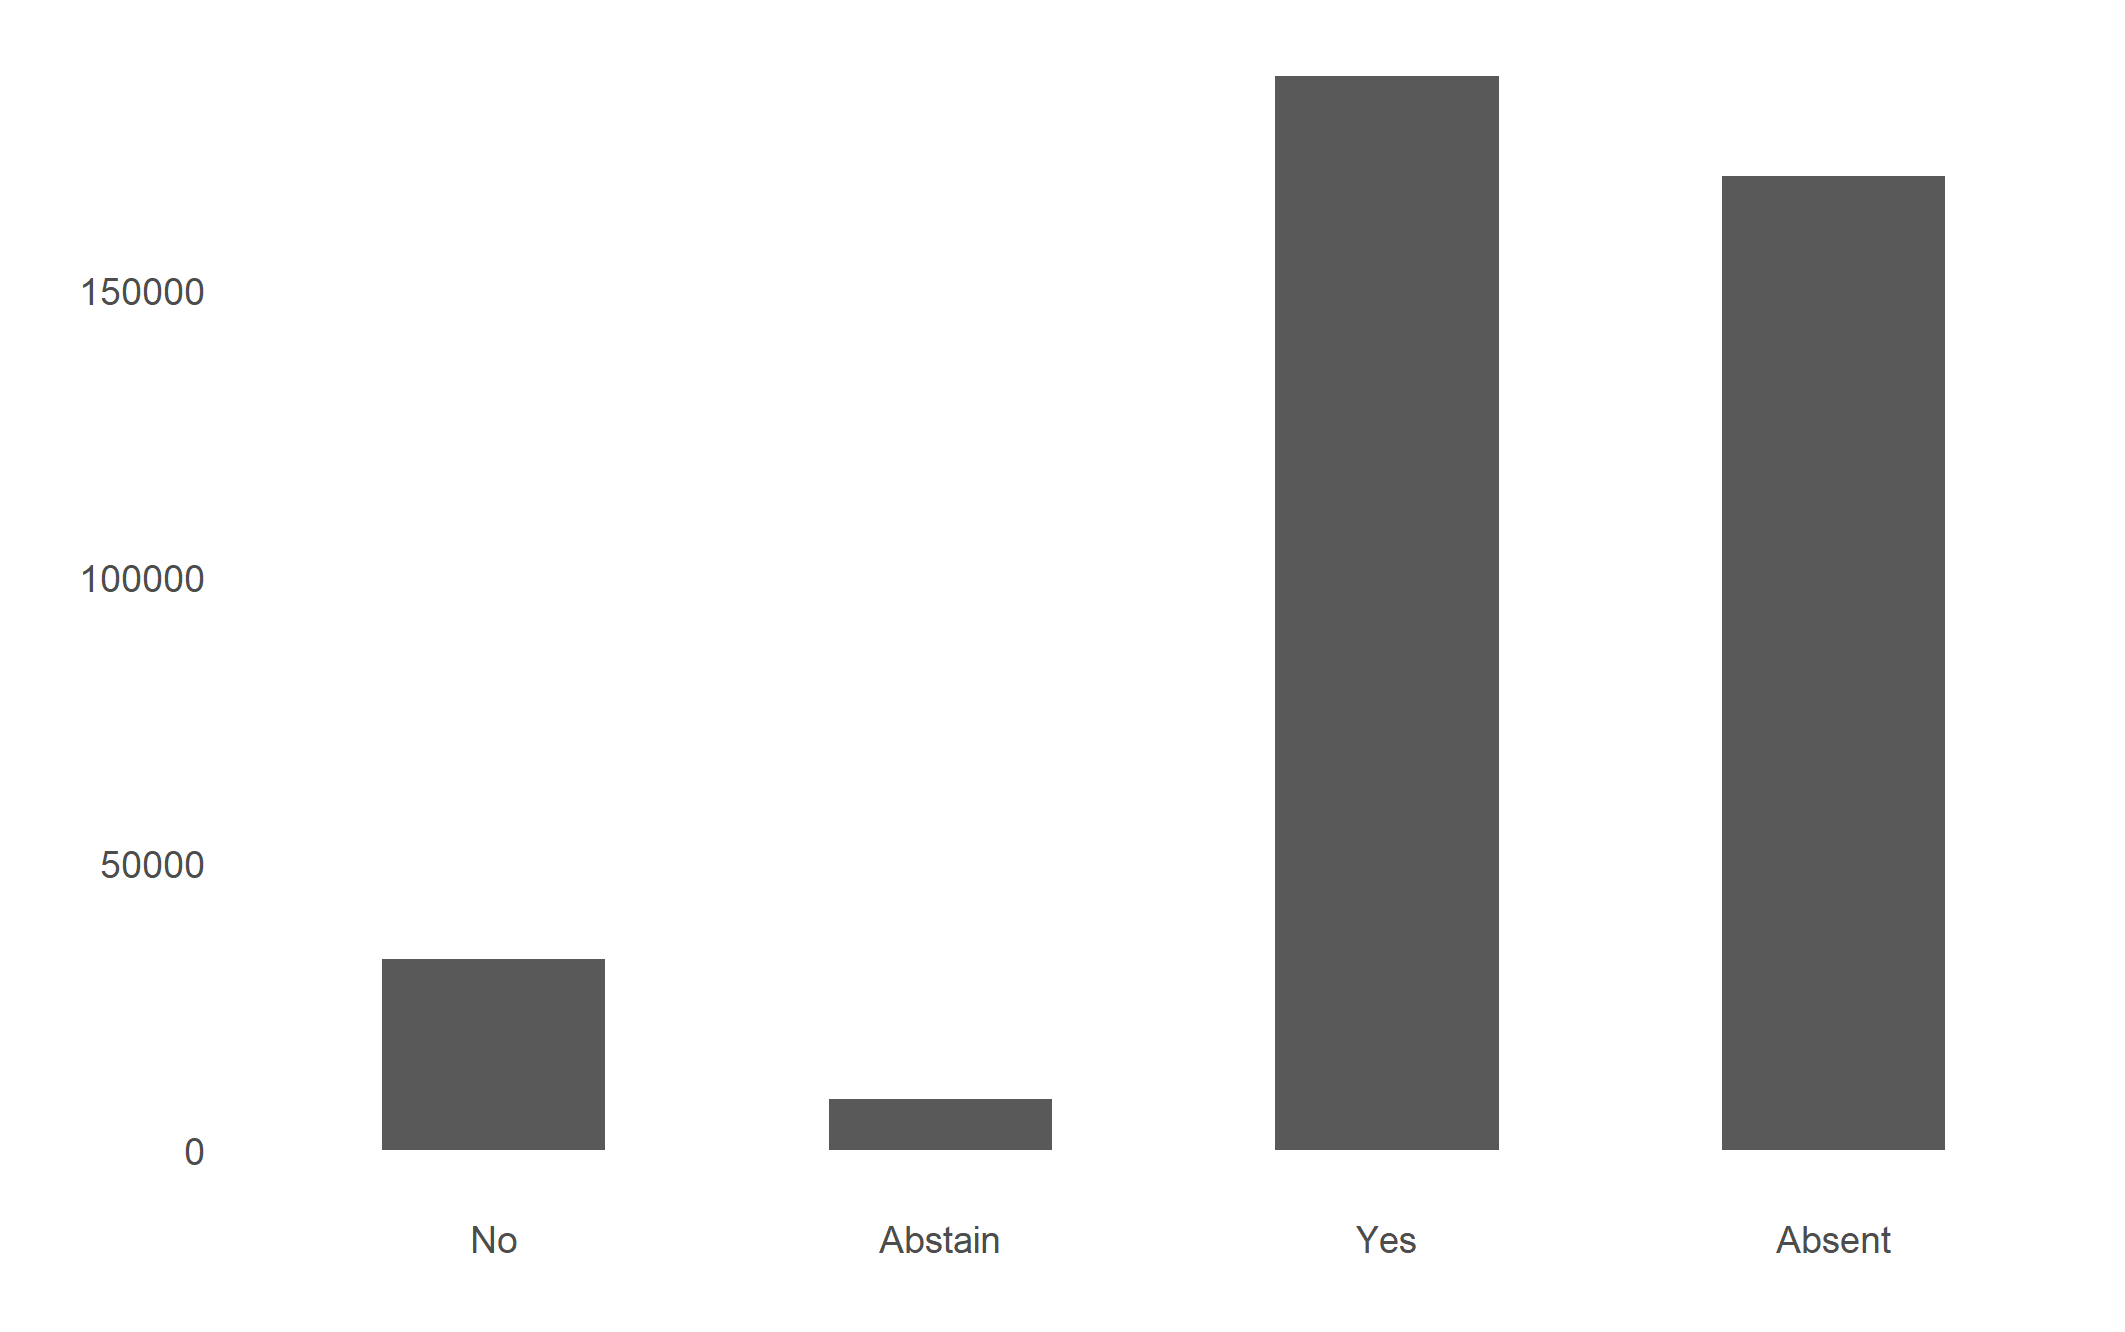
\includegraphics[width=.8\linewidth]{arp_hist}
	\end{figure}

	For this comparison, I only used the W-NOMINATE model as a reference point because the divergence in estimates makes examination of the differences more difficult with multiple models. Figure \ref{tunis_ideal} shows the absence-inflated estimates plotted against the W-NOMINATE estimates that only include bills with a relatively balanced proportion of yes and no votes. For this dataset, W-NOMINATE had to drop nearly half of the recorded votes because they did not have enough yes or no votes to estimate an ideal point.
	
	Unsurprisingly, Figure \ref{tunis_ideal} shows substantial heterogeneity in the estimates, especially for the left-hand side of the plot which shows the ideal point estimates of the governing coalition. The fact that ideal points differ for the governing coalition reflects the parliamentary nature of the legislature because these MPs presumably would abstain or be absent rather than registering a no vote. On the other hand, there is much more agreement in the models for the opposition on the far right tail, which is free to register no votes in response to government legislation. The confidence intervals for some MPs are extremely wide in the W-NOMINATE estimates, rendering the resulting ideal points effectively useless. In addition, there is overall more spread to the absence-inflated estimates, which is likely because of MPs using absences and abstentions to register their disagreement with coalition policy.
	\begin{figure}
		\centering
		\caption{Ideal Point Estimates for Tunisian Assembly of Representatives}\label{tunis_ideal}
		\includegraphics[width=\linewidth]{tunisia_arp_compare}
	\end{figure}

	Because this model estimates ordinal cutpoints, we can plot the abstention mid-points (i.e., the points where a legislator is indifferent at abstaining versus voting yes or no) over the legislator ideal points. Figure \ref{tunis_abst} shows these points for the Tunisian Assembly. In this vote, the absence midpoints are located in the center of the government's distribution of ideal points, which is an indication that abstention for this bill is primarily a way for MPs in the government to signal their disagreement. This plot also makes clear the limitations of the model: two cutting lines is not enough to capture all the reasons that an MP may choose to abstain on a particular bill. However, the intention of presenting this ordinal IRT is not to suggest that it does represent the full range of reasons for abstention, but rather that it is a solid foundation on which to build more complicated models that examine in-depth further aspects of legislative behavior.
		\begin{figure}
		\centering
		\caption{Abstention Indifference Points for Tunisian Assembly}\label{tunis_abst}
		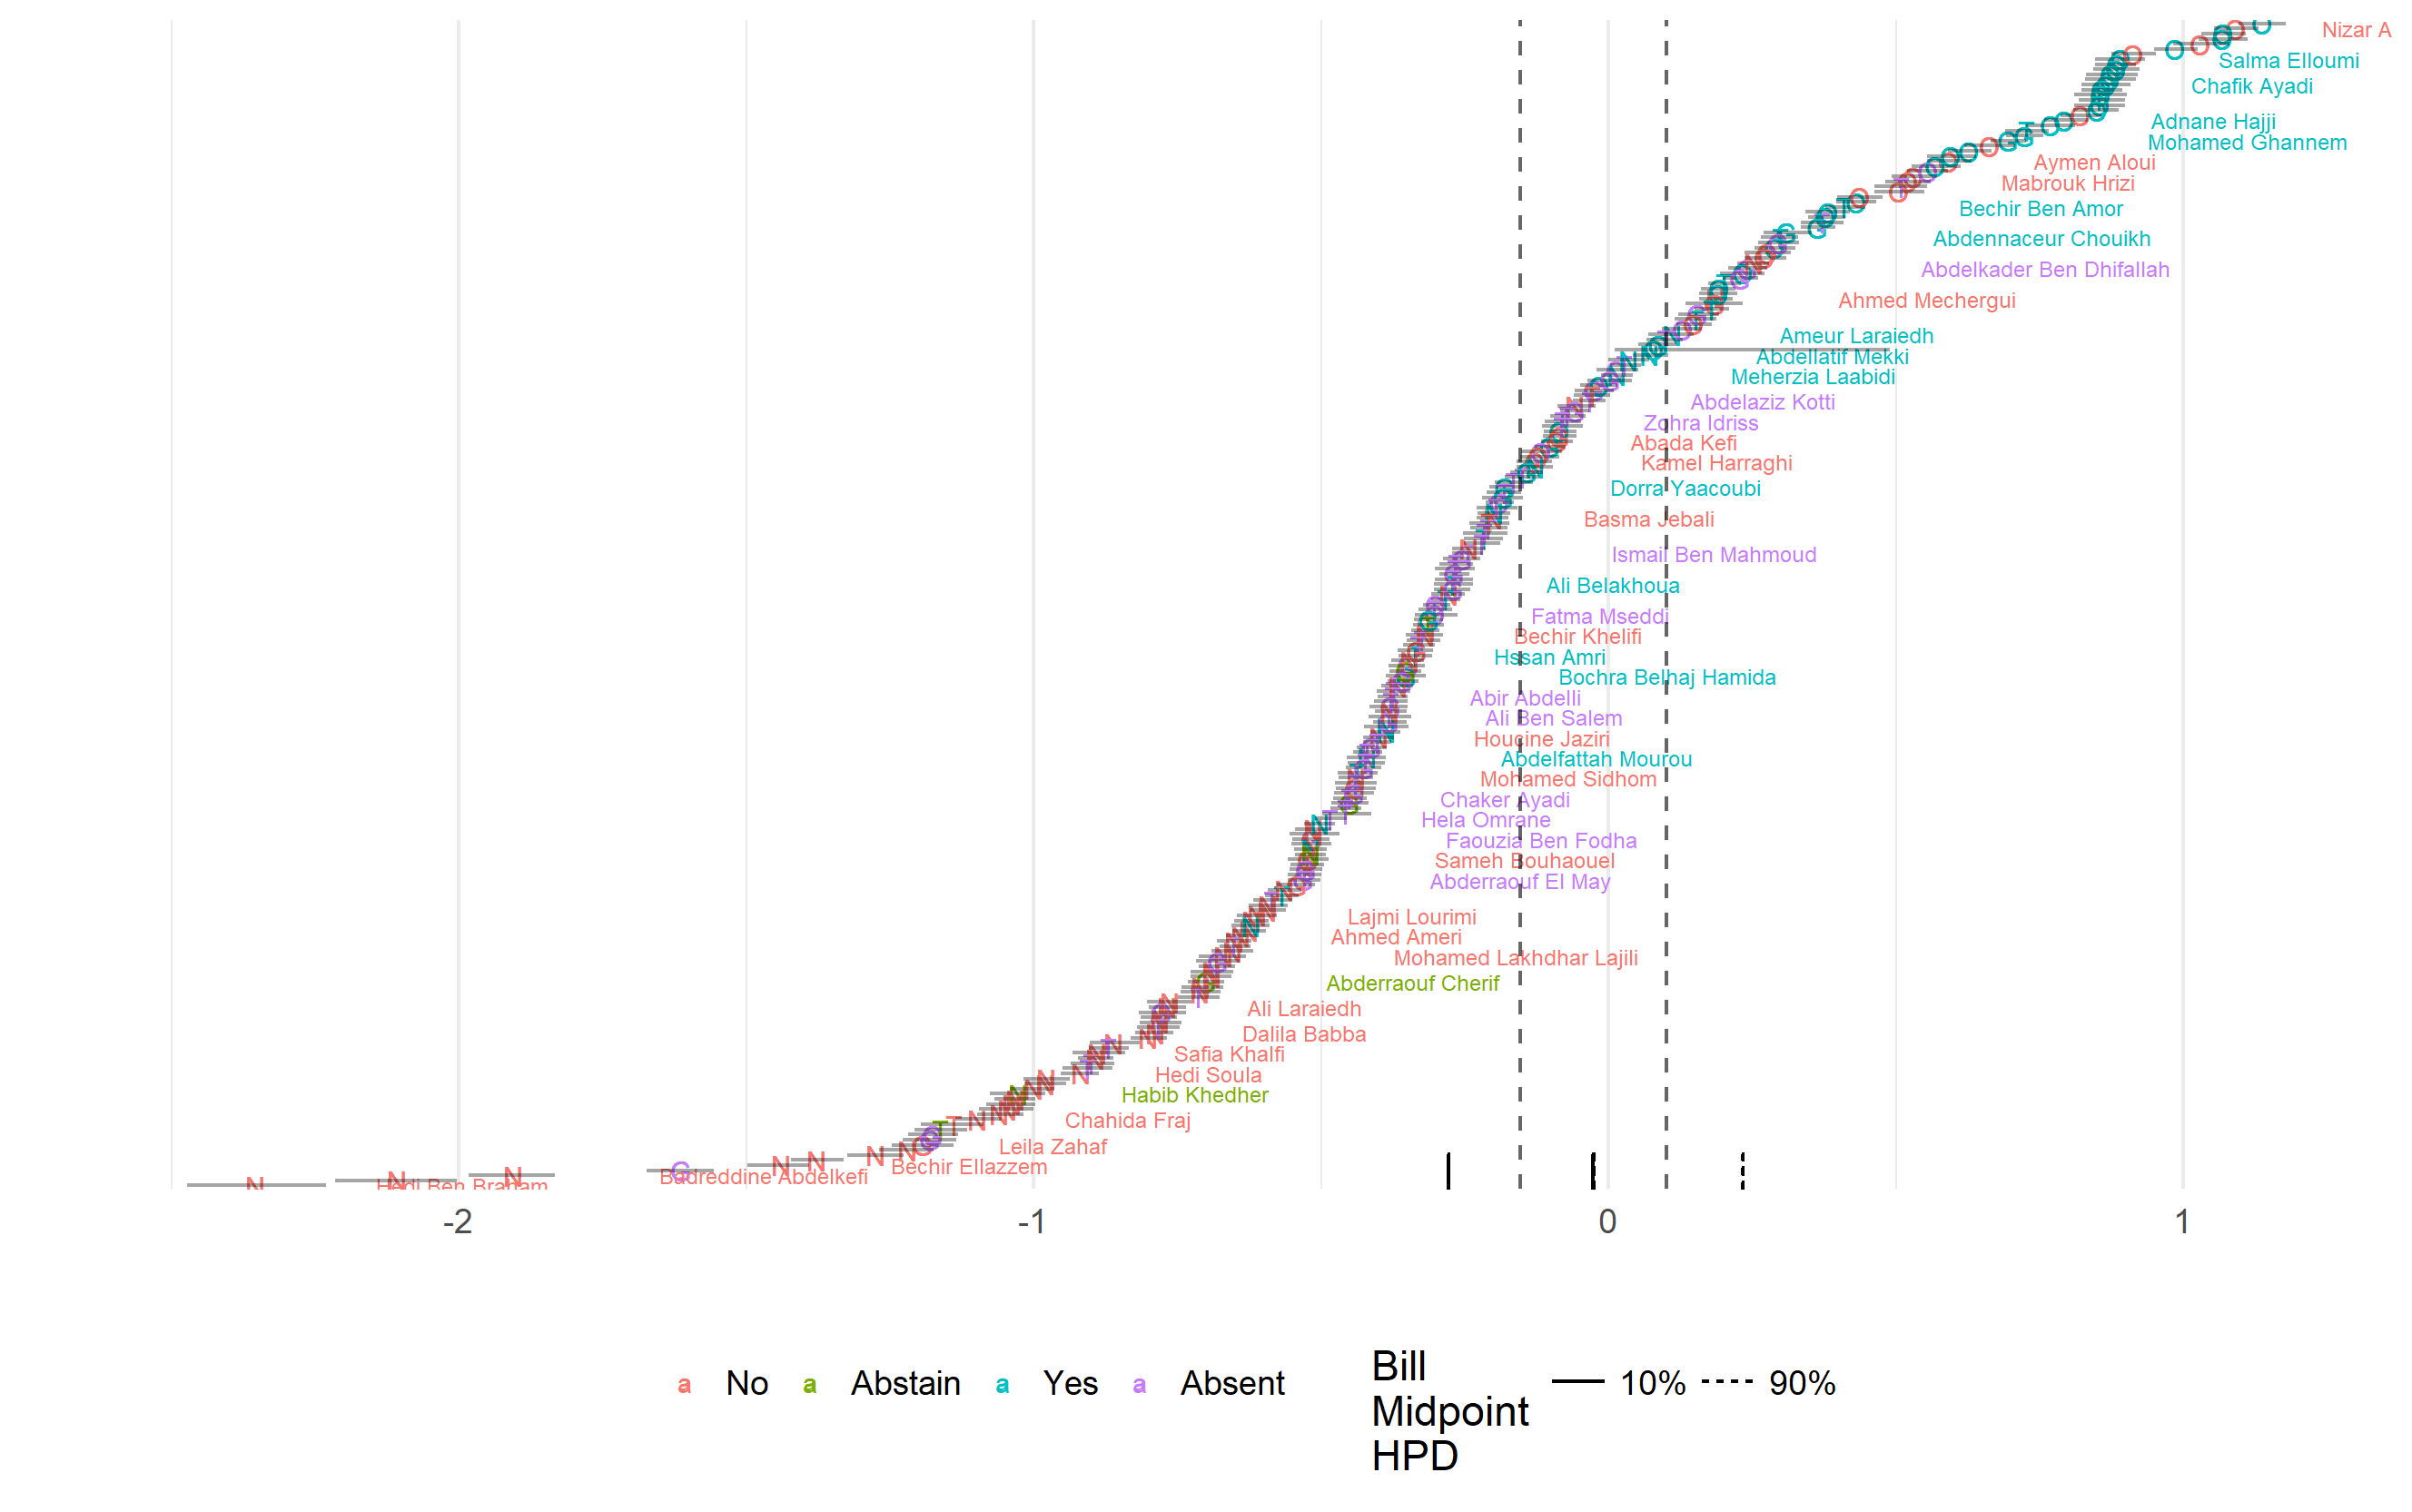
\includegraphics[width=\linewidth]{tunisia_abstain}
	\end{figure}
	
	\section*{Discussion}
	
	The aim of the absence-inflated model is to provide scholars with an ideal point estimation that can handle most recorded categories in voting data: absences, abstentions, yes and no votes. In theory and in practice, this methodology will improve ideal point estimates both by lowering uncertainty intervals but also by delineating strategic behavior that was previously treated as random or ignorable. The main innovation of this model is to treat absences as a kind of strategic action rather than missing data that must be imputed. Multiple imputation treats absences as containing no information about the ideal point distribution, and for that reason the missing values can and should be filled in with the true yes or no votes. This methodology, however, is unnecessarily restrictive when there is a known relationship between absences and votes: as the probability of absence increases, the probability of any vote decreases proportionally. This fact about the structure of legislative behavior is enough to create a model that incorporates all of the observed data. 
	
	The main limitation of the proposed method is the additional estimation cost. The form of the model presented can only be estimated via MCMC, which requires considerable time with larger datasets. However, part of this difficulty can be overcome with variational Bayesian estimation, which is also included in the R package \texttt{idealstan}. Variational Bayes estimates a stochastic approximation of the true posterior formed by reducing the posterior to a series of normal distributions. In general, variational Bayes tends to obtain correct mean of the posterior values, but it underestimates uncertainty \parencite{NIPS2015_5758}.
	
	In general, the estimation burden can be reduced by using variational Bayes to obtain initial estimates and then running a full Bayesian model when all of the modeling choices have been decided. Furthermore, \texttt{idealstan} utilizes variational Bayes for automatic identification of models by selecting posterior modes with an unidentified variational Bayes run. This step can save considerable time for the analyst by selecting the best bills or legislators to use to constrain the polarity of the model. 
	
	Although comparisons were made with the standard CJR and W-NOMINATE models, it is not the argument of this paper that these ideal point estimators should be avoided by practicioners. These ideal point models are accurate estimations of binary responses, and if the research question primarily focuses on yes and no votes, then these models are more parsimonious and a better fit to the available data.
	
	\section*{Conclusion}
	
	In this paper I presented an absence-inflated ideal point model that is capable of analyzing the full range of recorded outcomes in a legislature. Absences are addressed by deflating the probability of a legislator's vote choice by the probability that the legislator will choose to be absent on a given vote. This decision is modeled as its own ideal point decision-making process, in which legislators choose to be present when the absence point of the bill gives the legislator greater utility by showing up to vote. The estimation of this additional set of bill parameters provides new avenues for analysis of legislatures that explicitly examine strategic absences, such as US Congresspeople who are on the campaign trail.
	
	In addition, the model offers as well the ability to model abstentions as a separate vote category by utilizing an ordered-logit IRT framework. Abstentions, while relatively rare in the US Congress, are a common phenomenon in parliamentary legislatures where votes against the member's coalition are difficult, and abstention is a useful way to register disagreement with the majority group. The use of Bayesian estimation prevents the difficult problem of perfect separation in ordered logistic models so that the ordered choice IRT model can be used on legislatures with any number of abstentions.
	
	The aim of this model is to create a tool that scholars can use to immediately model the full set of recorded data about legislator behavior with regard to rollcall votes. The model does not address intra-party or intra-coalition dynamics, but rather provides a framework for finding the lowest-variance explanation of all observed legislator actions. The model builds on the foundation of ideal point models in political science, and the estimates should be comparable to existing approaches. Furthermore, all of the models presented, in addition to several extensions, are available in the R package \texttt{idealstan}.
	
	\printbibliography
	
\end{document}